\documentclass{article}

\usepackage[english]{babel}
\usepackage[a4paper,top=2cm,bottom=2cm,left=3cm,right=3cm,marginparwidth=1.75cm]{geometry}

\usepackage{amssymb}
\usepackage{amsfonts}
\usepackage{amsmath}
\usepackage{algpseudocode}
\usepackage{algorithm}
\usepackage{graphicx}
\usepackage{minted}
\usepackage{parskip}
\usepackage{pdflscape}
\usepackage{tcolorbox}
\usepackage{multicol}
\usepackage{tree-dvips}
\usepackage{qtree}
\usepackage{xcolor}
\usepackage[toc,page]{appendix}
\usepackage{multirow}
\usepackage[utf8]{inputenc}
\usepackage{hyperref}

\usepackage[colorlinks=true, allcolors=blue]{hyperref}
\usepackage{textcomp}

\title{Solving 2048 with Expectimax}
\author{David Cook}

\begin{document}
\maketitle
\newpage
\tableofcontents
\newpage
\begin{abstract}
This project aimed to make an optimised algorithm to solve a 2048 game using the expectimax algorithm. There are several key approaches I wanted to try to extend this. Firstly, I wanted to get my algorithm working on $n \times m$ games of 2048. Despite this, the project\textquotesingle s main focus is getting good performance on a $4 \times 4$ game, as there is more data to evaluate the game\textquotesingle s performance. Various techniques, most effectively multi-threading, have been tried to optimise the maximum score that can be achieved.

Many previous solutions of this project have been unable to get past 4096 reliably using the expectimax algorithm. Early on in this project, 4096 was also the maximum value that could be achieved in a reasonable amount of time. The introduction of multi-threading was the main advantage that allowed this implementation to reach 8192 with reasonable constancy.

For a demo of the program produced, see Appendix~\ref{subsec:vid}.
\end{abstract}
\section{Introduction}
\label{sec:intro}
\subsection{The Problem}
\label{subsec:problem}
2048 is a game which features a 4x4 grid containing powers of 2. Each game starts with two cells, with a value of either 2 or 4.
All the tiles can be slid in any of the four directions (up, down, left and right); all the tiles can move simultaneously. When two of the same powers of 2 collide, the tiles merge, creating the next power of 2. The new tile increases the score by its new value. After each move, a new tile (either 2 or 4) will appear in a random free cell~\cite{game2048}.

This project aims to play a 2048 game using an AI search algorithm. Some previous projects have reached the tile of 32k\cite{_16k2048ai}. Reaching 32k is uncommon; many implementations can only reach 4096~\cite{aiplays2048,expectimax2048}.

A promising search algorithm is expectimax (see section \ref{subsec:automated_techniques})/ This algorithm is designed for scenarios where there are two agents, one making random decisions and one making rational decisions~\cite[~p.200]{russell2010artificial}. In some situations, it is possible to pre-compute a decision tree, saving execution time.
Pre-computing a traditional 2048 decision tree is impractical, particularly when factoring in variable-size games.

Expetimax is also the algorithm used by \cite{_16k2048ai}, the implementation capable of reaching a tile of 32k; however, it does not have much accompanying documentation. It is difficult to understand what is happening.

Some optimisations could be applied to the expetimax algorithm to improve the performance restraints caused by this project's complexity. Due to the time constraints of this project, there was not enough time to test all of these approaches.
\begin{itemize}
    \item Pruning unlikely possibilities.
    \item Pruning moves that are likely to be poor decisions.
    \item Dynamic Depth: When fewer possibilities exist, the tree can be searched to a greater depth.
    \item Multi-Threading: Expectimax is a relatively simple algorithm to implement multi-threading with.
    \item Memorisation: Prompted by my \cite{_16k2048ai}, I discovered there are actually a reasonable number of repeated nodes in a 2048 tree; only calculating entire branches of the 
    tree once may be significant.
    \item Using a good heuristic.
\end{itemize}

\subsection{Deliverables}
\label{subsec:deliverable}
\subsubsection{Proof of concept programs}
\begin{enumerate}
    \item Decision Tree
    \item Simple Expectimax Example
    \item 2x2 2048 Game
    \item 2048 with a heuristic
\end{enumerate}
\subsubsection{Report}
\begin{enumerate}
    \item Professional Issues: Licensing. (interim report)
    \item Design patterns in AI search. (interim report)
    \item Techniques used by humans and previous automated solvers. (interim report)
    \item User interface design for the solver. (interim report)
    \item Complexity and big $O$ notation. (interim report)
    \item The practicality and the effectiveness of the pruning expectimax tree.
    \item The heuristics have been generalised to support more 2048 games.
    \item Describe interesting algorithms and programming techniques, such as expectimax, used in the project.
    \item Implementation and performance of the decision tree.    
\end{enumerate}
The report will describe the implementation and optimisations of the expectimax algorithm, focusing on any software engineering principles used in the processes. 
\subsubsection{Final Program}
The final program will:
\begin{enumerate}
    \item Be written in java, with a full Object-oriented design, using modern software engineering principles.
    \item Be theoretically capable of playing any $n \times m$ 2048 game, though eventually break down due to performance.
    \item Have a user interface capable of keeping track of stats about the algorithms and an easy way of creating new $n \times m$ games.
\end{enumerate}
\newpage
\section{Proof of Concepts}
\label{sec:proof_of_concepts}
\subsection{Decision Tree}
\label{subsec:dt}
There are many ways to implement a tree structure; various are more appropriate than others. The operations that are required in this situation are \cite{russell2010artificial}:
\begin{itemize}
    \item Generate a tree from the root node.
    \item Transverse the entire tree to calculate the score.
    \item Walk to a direct child node and regenerate the tree.
\end{itemize}
In the latter case, the scores  must be regenerated on the pre-existing nodes and some new nodes node to generate.
I will assume generating a node can be done in $O(1)$ time; however, this may not be true. Generating or traversing nodes in a tree with $n$ nodes can not be done in $O(n)$ time. Reading a direct child can not be done in $O(1)$ time.

A common approach to making a tree is using a simple node class such as:
\begin{minted}{java}
public class Node {
    float score;
    Node[] children;
}
\end{minted}
This is a node with an array of references to its child nodes. Traversing this entire tree will have a time complexity of 
$O(n)$. Arranging these nodes into a tree structure takes $O(n)$ and finally picking a direct child of a node takes $O(1)$,
This simple tree implementation is adequate for the job, so more complex tree solutions are unnecessary.

See Appendix \ref{subsubsec:apendixdt} for full code.
\subsection{Expectimax}
The expectiminimax algorithm allows games to play with two rational agents and an element of chance \cite[p.~200]{russell2010artificial}. A simplified version of this algorithm, using only one rational agent, called expectimax, can perfectly model a game 2048. I intended to create an arbitrary expectimax tree and calculate the scores of each node.

\label{subsec:expectimax}
\begin{figure}
    \centering
    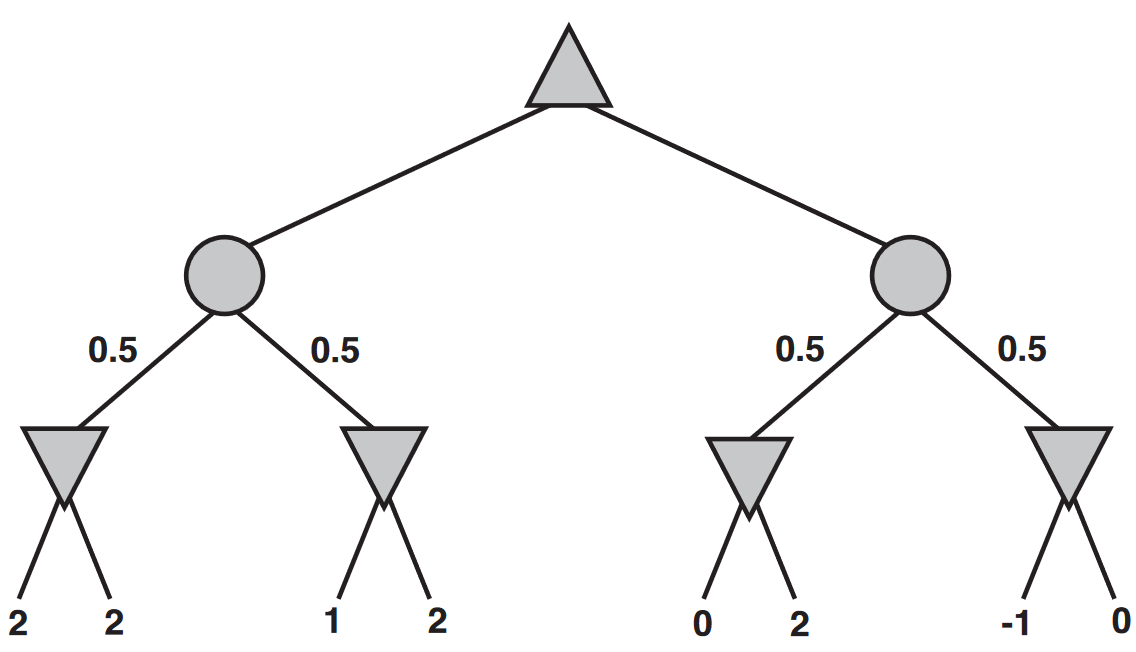
\includegraphics[width=0.7\textwidth]{expectimax.png}
    \caption{An expectiminimax tree example \cite[p.~200]{russell2010artificial}}
    \label{fig:expectree}
\end{figure}
The decision tree required in the expectiminimax algorithm (Figure \ref{fig:expectree}) has four types of nodes. However, three nodes are needed for the problem of solving 2048. These three types of nodes include:
\begin{itemize}
    \item Terminus nodes: These nodes are the leaves of the tree. Their score is already known and used to calculate the score in the rest of the tree.
     \item Chance nodes: These nodes represent situations where random states may follow. The weights between
    a chance node and its children represent the probability of that event occurring. A chance node\textquotesingle s score is the weighted sum of its children.
    \item Maximising nodes: These nodes take the score of the maximum-scoring child.
    \item Minimising nodes: These nodes take the score of the minimum-scoring child (Not used in this project).
\end{itemize}

Figure \ref{fig:expectree} has an example expetiminimax tree. To calculate the best move to be made from the root node, we would first evaluate the two leftmost minimising nodes. These would score $2$ and $1$, respectively.
Next is the leftmost chance node, which takes the average value of its children, $1.5$. This is then repeated for the rightmost sub-tree, the minimising nodes score $0$ and $-1$, respectively and there parent chance node score $-1.5$. The highest scoring move that can be made from the right move it therefore left.

Each of these three relevant types of nodes has been converted to individual java classes, caching the scores in a float
attribute, so they only need to be calculated once.
For the complete code for this proof of concept, see Appendix \ref{subsec:apendixexpecti}

\subsection{2048}
\label{subsec:2048}
This proof of concept was primarily created using one source \cite{source2048}, the original 2048 source code. While not
directly copying any code, relevant features are based on the original code. This has also been adapted to support any $n \times m$ game.

This prototype helpfully highlighted some behaviours to avoid when implementing the final version.
\begin{itemize}
    \item If you loop over the numbers in the wrong order, a tile may collide with a tile that will be moved later. 
    See Figure \ref{fig:slidebug} for an example.
    \begin{figure}
        \centering
        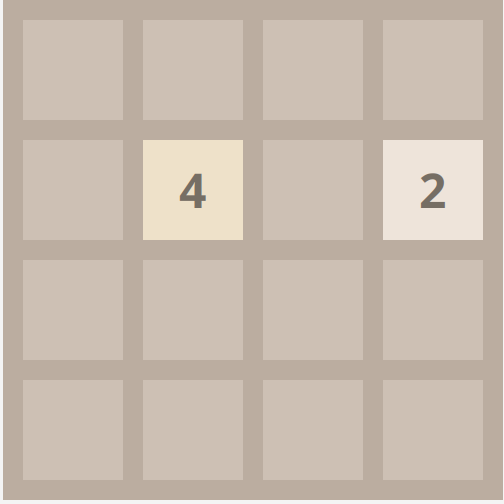
\includegraphics[width=0.3\textwidth]{2048_slide.png}
        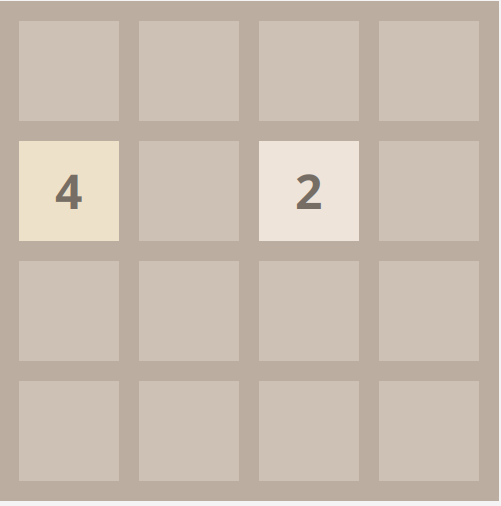
\includegraphics[width=0.3\textwidth]{2048_slide2.png}
        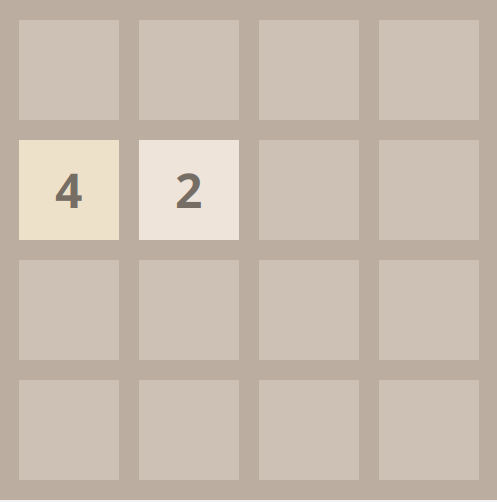
\includegraphics[width=0.3\textwidth]{2048_slide3.png}
        \caption{The first image shows a state before a left slide, the second one after an incorrect left slide, and the third one after a correct left slide.}
        \label{fig:slidebug}
    \end{figure}
    \item When merging tiles, you must ensure that you do not merge a tile multiple times. See Figure \ref{fig:mergebug} for an example.
    \begin{figure}
        \centering
        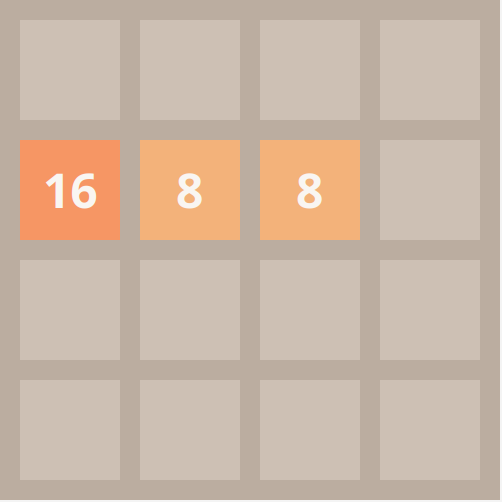
\includegraphics[width=0.3\textwidth]{2048_merge.png}
        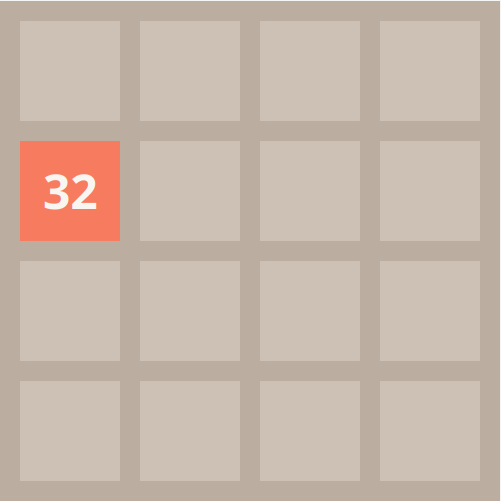
\includegraphics[width=0.3\textwidth]{2048_merge3.png}
        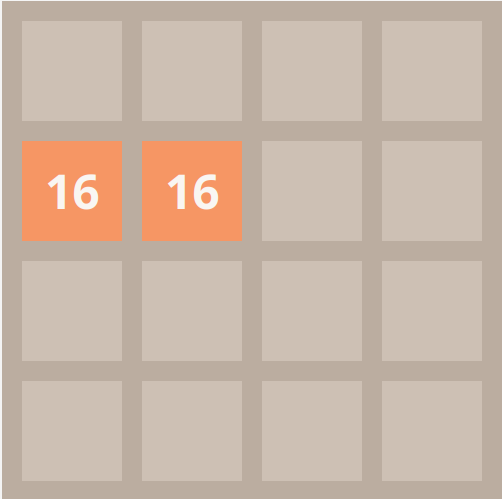
\includegraphics[width=0.3\textwidth]{2048_merge2.png}
        \caption{The first image shows a state before a left slide, the second one after an incorrect left slide, and the third one after a correct left slide.}
        \label{fig:mergebug}
    \end{figure}
\end{itemize}
The test suite picked up the first issue; however, I had not considered the second case before writing the proof of concept. I only caught the second issue because I wrote a command line user interface (see figure \ref{fig:2048_cli}), allowing me to play the game and pick up on bugs. 
    \begin{figure}
        \centering
        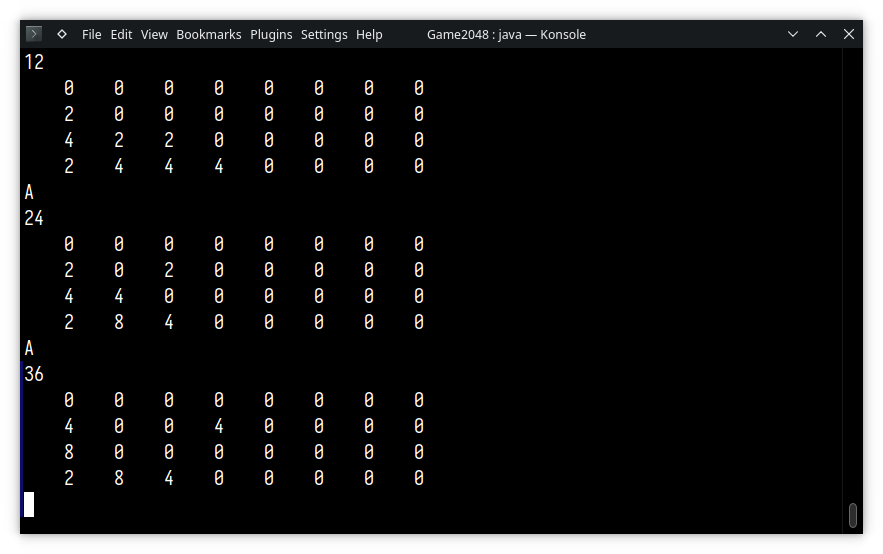
\includegraphics[width=0.8\textwidth]{Screenshot_20221201_231121.png}
        \caption{Command line user interface used by 2048 prototype playing a 4 x 8 game.}
        \label{fig:2048_cli}
    \end{figure}
    For full proof of concept, code see Appendix \ref{subsec:apendix2048}
\subsection{2048 with Expectimax}


\label{subsec:2048_expectimax}
A working prototype of expectimax has been developed (see \ref{subsec:expectimax}). A working 2048 prototype has already been developed (see \ref{subsec:2048}).  These components need to be modified to apply the expectimax algorithm to the 2048 game. 
The aim is to generate the full tree instead of using a heuristic, but to do this, the 2048 puzzle must be simplified.

Two modifications were made to the setup of 2048 to ensure the tree was a reasonable size:
\begin{itemize}
    \item Make the game $2 \times 2$.
    \item After a move, only the number 2 can appear.
\end{itemize}
With these modifications, there are at most only three possible free cells where a tile can be added. With possible moves, the tree can only grow by $3 \times 4 = 12$ for each move.
A traditional 2048 game has four possible moves and 15 possible free cells where a tile can be added, meaning the tree can grow by $15 \times 4 = 60$ for each move.

Originally the only modification to the game was making it $2 \times 2$ to increase the tree by $6 \times 4 = 24$ for each move. However, the prototype could not calculate the tree within a reasonable time. Hence, the new tiles are limited to just the '2' tile to reduce the complexity further.
For complete code for this proof of concept, see Appendix \ref{subsec:apendixauto2048}
\subsection{Heuristic for 2048}
\label{subsec:heuristic}
In this prototype, the restrictions were removed from the game. The size of the game is now $n \times m$, and either a $2$ or $4$ can appear in the grid. This makes it impracticable to calculate the full tree. To do this, an arbitrary  %depth% limit is chosen for the tree. At the leaf nodes in the tree, a heuristic value is calculated.

Two different heuristic functions were implemented.
\begin{itemize}
    \item Sum up all the items in the grid. This was a simple heuristic to ensure that the algorithm worked as expected. This heuristic could not achieve high scores.
    \item Sum up all the values multiplied by the row they are in (Top row = 1 and bottom row = n). The most rewarding path was placing larger numbers lower in the grid.  This heuristic was much more effective, reaching a tile of 512.
\end{itemize}

With this, the algorithm can theoretically be applied to any 2048 game, which becomes impractical for a large $depth, n$ or $m$. The original plan was to apply this to a 2x2 game; however, due to the nature of the heuristics, I removed this requirement and allowed any grid size, as the $depth$ limit makes this practical. For the complete code see Appendix \ref{subsec:apendix2048H}.
\section{User Interface Design}
\label{sec:ui}

The user interfaces resemble the original 2048 game, as shown in Figure~\ref{fig:2048interface}.
Parts of the user interface are appropriate for my solver. However, some features must be removed.

\begin{figure}
    \centering
    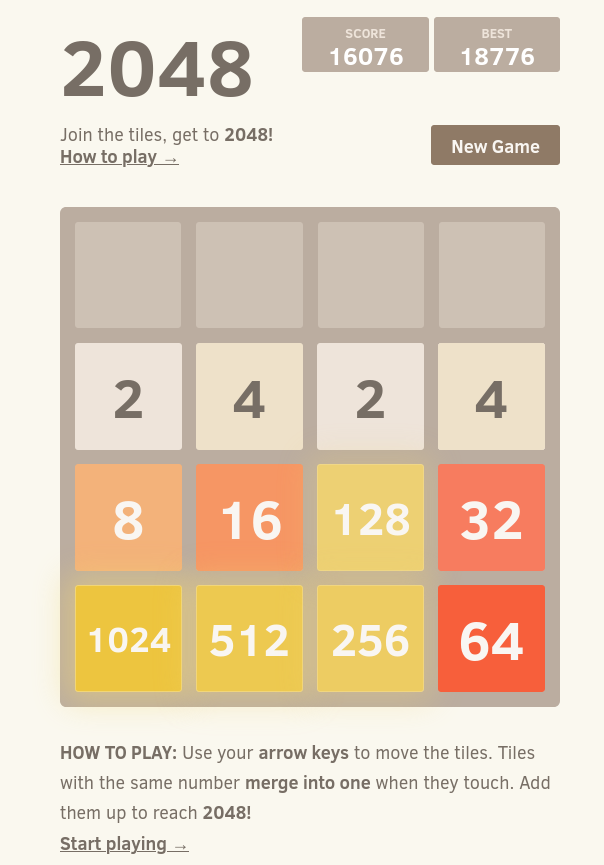
\includegraphics[width=0.4\textwidth]{2048-interface.png}
    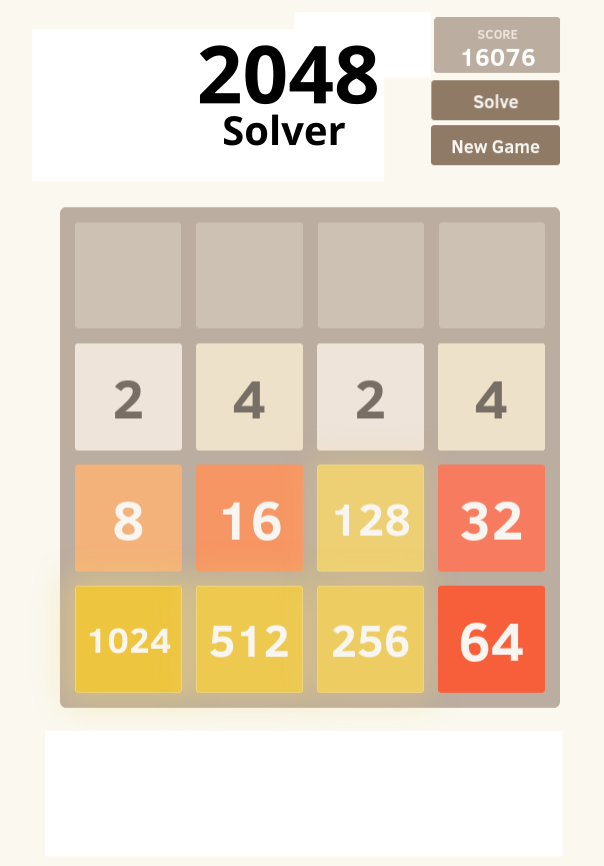
\includegraphics[width=0.4\textwidth]{interface-mockup.png}
    \caption{On the left is a screenshot of the official 2048 user interface \cite{game2048} and on the right
    is an edited version of this image designed to represent what my main interface might look like}
    \label{fig:2048interface}
\end{figure}

Firstly the instructions on how to play the game seen at both the top and bottom of the page have been removed
as the game will play itself. Secondly, a new solve button has been added.

The 'best' score box has been removed from the interface. I will need to keep track of more data than the best score to evaluate how effective the algorithm is and will likely log this in a CSV file.

Most versions of 2048 have an animation that plays as the tiles slide; while this would be possible, as animations do exist in JavaFX \cite{javadocfx}, I am not familiar with them and think it is not worth the time to re-implementing the animations.

When creating a new game, it is important that the user can enter the size of the new game; however, this input should not be visible when the user doesn\textquotesingle t want to make a new game. A long-established solution is providing the user with a popup dialogue asking for the size of the game. There is no reference for this in the original 2048 to base the user interface on, so instead of modelling an existing interface, I have created a mock-up of what the interface should look like figure \ref{fig:popup}

\begin{figure}
    \centering
    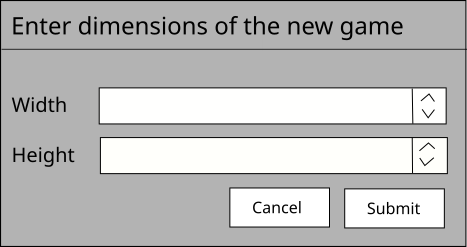
\includegraphics[width=0.4\textwidth]{newGamePopup.png}
    \caption{Mock up of the new game popup window.}
    \label{fig:popup}
\end{figure}
\section{Design Patterns for AI Search}
\label{sec:dp}
There are many ways design patterns can be used in AI search algorithms, specifically in the expectimax algorithm. Figure \ref{fig:alg_uml} shows the structure of the code used for the algorithm; a few changes have been made that have not yet been implemented.


\subsection{Factory Design Pattern}
\label{subsec:factory}
A factory design pattern is a creational design pattern used to hide the complexity of creating an instance of a class \cite{CS2800_creational}. The original implementation of the expectimax algorithm includes three types of nodes:
\begin{itemize}
    \item \mintinline{java}{MaxNode}
    \item \mintinline{java}{ChanceNode}
    \item \mintinline{java}{LeafNode}
\end{itemize}
The  expectimax tree will always start with a maximising node. This means that despite the complexity of the Node classes, given a game state and the maximum depth of the tree, it is very simple to create the root node of the initial tree. Generating the child nodes is slightly more complex than the initial root node. Depending on the parent and if the node has children, it can be any of the three node types. For this, two creational methods can be created. One is to create an initial root node that only takes in a small amount of information and one that is package private that takes in more data to determine what type of node it is.

Since implementing multi-threading, the process of making nodes is slightly more straightforward. There is one node class \mintinline{java}{Node}. Its behaviour comes from a class implementing the \mintinline{java}{NodeBehaviour} interface. See section \ref{subsec:state} for more about this.


\subsection{State Design Pattern}
\label{subsec:state}
A state is a behavioural design pattern used when an object\textquotesingle s behaviour needs to change based on some condition \cite{CS2800_behavioural}. A class using that state design pattern has an attribute that will be referred to as \mintinline{java}{objectState}. \mintinline{java}{state} will have the type of some interface or superclass. When the 'state' of the object is changed, the \mintinline{java}{objectState} is changed to a different implementation of the interface. Any features of the class that depend on the state are delegated to the concrete implementations of this interface.

The state design pattern is used in the \mintinline{java}{Node} class. Each node has a behaviour which manages what happens when a heuristic is applied to the node, when the next node is requested and manages the node's children. Every node starts as a \mintinline{java}{LeafNodeBehaviour} which has the following features:
\begin{itemize}
    \item Stores no data related to children; it is known their aren\textquotesingle t any.
    \item \mintinline{java}{nextNode (Heuristic)} simply throws EndOfGameException. This relies on the assumption that the tree has a depth of at least two.
    \item \mintinline{java}{applyHeurstic(Heuristic)} applies the heuristic to the games state.
\end{itemize}

There are two other behaviours \mintinline{java}{NodeBehaviourMaximize} \mintinline{java}{NodeBehaviourChance}. Each stores child nodes in an array, applying the heuristic to their child nodes, taking the most significant or weighted average value. The following node method will make the best move or pick a random one.

When \mintinline{java}{generateChildren(...)} is called on a node, an appropriate Node Behaviour will be generated (based on a method passed to the constructor), and the node 'state' will be switched to this new behaviour.

For a UML diagram see Appendix \ref{subsec:apendixns}.

\subsection{Singleton Design Pattern}
\label{subsec:singleton}
A singleton is a creational design pattern that ensures at most one class instance; if an object is required multiple times, the same object is returned each time \cite{CS2800_creational}.

The most clear-cut case for this design pattern is the heuristic classes. Apart from the Dynamic Snake and Fail Wrapper heuristics, none of the heuristics takes any attributes. This is an obvious example of where implementing a singleton design pattern would be a good idea. If multiple instances of a heuristic are made, they would be precisely the same.

For UML Diagram, see Appendix \ref{subsec:apendixVS}
\subsection{Observer Design Pattern}
\label{subsec:observer}
An observer is a behavioural design pattern that is particularly useful when something needs to happen in an object based on an event in another object.
A typical example of where this design pattern can be used is event handlers in a user interface \cite{CS2800_behavioural}.

An observer interface consists of one function, often called \mintinline{java}{notify()}, or \mintinline{java}{update()}. This function is called by an observable object when some event occurs.

In this project, a class called \mintinline{java}{Solver} contains the code for the expectimax algorithm. Each time it calculates and makes, a move, this needs to be updated in the View. To make
this happen, an observer design pattern is used. Each time the observer is notified, it includes a parameter that describes the game's current state, which is passed to the view to be displayed.
\subsection{Visitor Design Pattern}
\label{subsec:visitor}
Allows some processing to be done externally from the object (A). A second object (B) can visit object A, which accepts object B and finally runs the process on object A.  This is particularly uLeafNodefseful when there are multiple ways something can be evaluated or multiple things to be evaluated \cite{CS2800_behavioural}.

To be practical, the expectimax algorithm applied to 2048 requires a heuristic function. There are many different heuristic functions, and there may be various reasons to use one over another in certain scenarios; it is convenient to separate the heuristic code from the \mintinline{java}{GameState} and apply the correct heuristic function when needed.

For UML Diagram, see Appendix \ref{subsec:apendixVS}

\section{Techniques used to solve the game}
\label{sec:techniques}

\subsection{Human Approaches}
\label{subsec:human_techniques}
It can be difficult to automate a human strategy. However, it is possible to reward or penalise certain states, and human strategies can be a good place to start when looking for features to reward or penalise.

One human strategy is to keep the largest number in a corner and have a gradient leading to the smaller values like in figure \ref{fig:gradient} \cite{strategy2048}. In testing, this way of arranging the grid makes it relatively easy to merge multiple tiles in a few moves and reduces the risk of trapped values. However, it does lead to many duplicate values that are difficult to merge, so there is often insufficient space to reach the larger tiles.

\begin{figure}[!tbp]
    \centering
    \begin{minipage}[b]{0.45\textwidth}
        \centering
        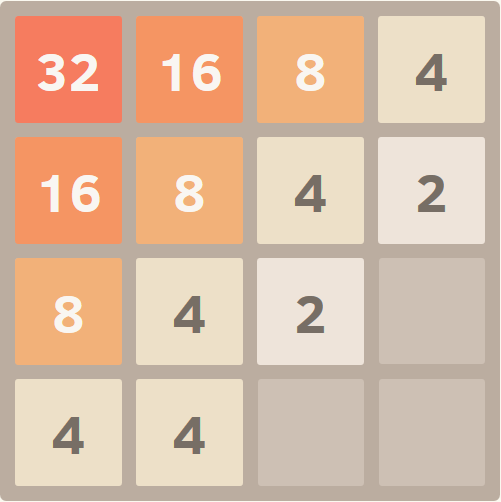
\includegraphics[width=0.5\textwidth]{gradient.png}
        \caption{Gradient pattern used in a 2048 human strategy \cite{strategy2048}.}
        \label{fig:gradient}
    \end{minipage}
    \hfill
    \begin{minipage}[b]{0.45\textwidth}
        \centering
        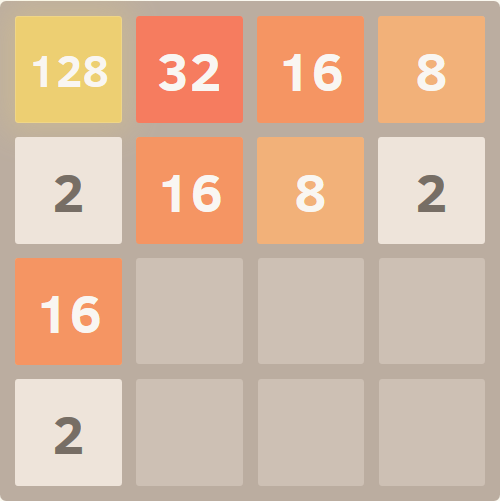
\includegraphics[width=0.5\textwidth]{trapped.png}
        \caption{Example of a trapped value in 2048 \cite{strategy2048}.}
        \label{fig:trap}
    \end{minipage}
\end{figure}
A trapped value is surrounded by larger numbers \cite{strategy2048}, such as the 2 in figure \ref{fig:trap}. Partially when there are not very many free cells around, these cells can be very difficult to get rid of and can take up useful space. They often appear when an empty tile is created after a merge in an area with large numbers. 

\begin{figure}
    \centering
    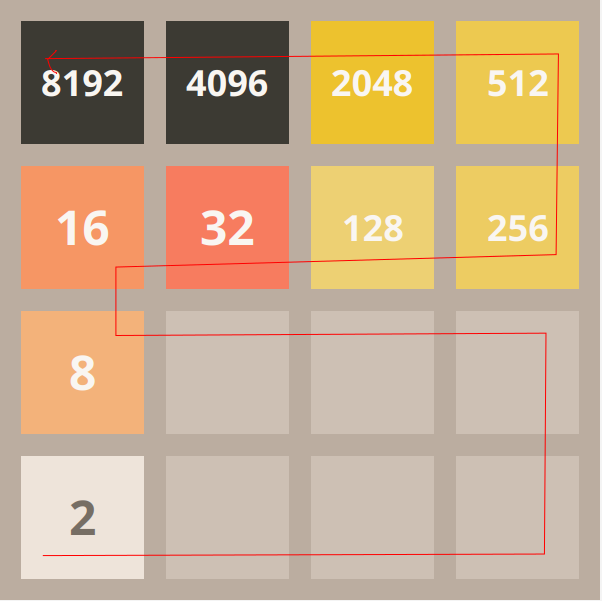
\includegraphics[width=0.2\textwidth]{bitmap.png}
    \caption{Snake pattern.}
    \label{fig:snake}
\end{figure}

Another approach is to try and order the tiles into ascending order using a snake shape (Figure \ref{fig:snake} \cite{aiplays2048}. The source for this approach describes an automated method; however,
humans can also use this. This was found to be a very reliable strategy in testing, even reaching tile 8192. The main drawback of this approach was that when merging the row with the largest numbers, there is a risk of producing a trapped value. With careful planning and some luck, it is possible to recover from these states.
\subsection{Automated Approaches}
\label{subsec:automated_techniques}
Many algorithms can be used to solve 2048, to varying degrees of success. Some of these algorithms are \cite{approches2048}:
\begin{itemize}
    \item Minimax - assumes that two rational agents always make their most optimal move \cite{minmaxCS2910}, this strategy does not adapt very well to 2048, according to \cite{approches2048} when citing \cite{minmax2048}.
    \item Expectimax - This is a much more effective strategy, similar to Minimax; however, the second agent is assumed to make random decisions \cite[p.~200]{russell2010artificial}. This model lends itself much better to 2048 as it exactly matches what happens \cite{expectimax2048}.
    \item Monte-Carlo Tree-Search - "Produces asymmetric trees, effectively pruning poor paths allowing for deeper searching on paths with greater potential." \cite{approches2048}. This method was highly effective compared to Mini-max and Expectimax.
    \item Average Depth-Limited Search - "ADLS approximates expectimax by running multiple simulations; it does not try to calculate all possibilities. Instead, likely outcomes will repeat more often." \cite {approches2048}. This method was highly effective.
\end{itemize}
While there are many different algorithms, some can be very effective; this report will focus on the expectimax algorithm. This is a relatively simple but effective algorithm \cite{expectimax2048}. As discussed in section \ref{subsec:2048_expectimax}, calculating an expectimax tree for even a small 2048 game is normally impractical; for a traditional 2048 game, there are even more possibilities, leading to an even bigger complete expectimax tree. Previous projects have used a depth-limited expectimax tree \cite{aiplays2048}, sometimes even with a dynamic depth \cite{expectimax2048}.

A heuristic function is needed to evaluate how good a state is at the end of the tree. Two interesting heuristics will be covered in this section. 

\subsubsection{Snake Heuristic}
\label{subsec:snake}
The snake heuristic is based on the most effective heuristic in \cite{aiplays2048}.

This heuristic works by calculating a weighted sum of the values in the grid:
\[
    \text{Let }S\text{ be the state of the game, }W=\begin{bmatrix}
    4^{15}&4^{14}&4^{13}&4^{12}\\
    4^8&4^9&4^{10}&4^{11}\\
    4^7&4^6&4^5&4^4\\
    4^0&4^1&4^2&4^3
    \end{bmatrix} \]\[\text{and }h(S)\text{ be the heuristic function.}
\]\[
    h_1(S)=\sum_{i=1}^{4}\sum_{j=1}^{4}W_{i j}S_{i j}
\]

This heuristic takes the human strategy of organising into snake shape rewards boards where this strategy has been applied.
\subsubsection{Diagonal Heuristic}
\label{subsubsec:diag}
The diagonal heuristic is used in the project \cite{expectimax2048}.
Similar to the snake heuristic, part of this is a weighted sum. However, there is also a penalty.

The penalty function $p(i, j) = \sum |\text{difference between each nonzero neighbour}|$. 
For example, with the grid state:
\[
\begin{bmatrix}
128 & 64 & 32 & 16 \\
8 & 32 & - &- \\
32 & 16 &8 &-
\end{bmatrix}\]\[
P(2, 2) = |32 - 64| + |32 - 16| + |32 - 8| = 32 + 16  + 24 = 72
\]

The heuristic function, where $S$ is the games state, and
$
W=\begin{bmatrix}
    6&5&4&1\\
    5&4&1&0\\
    4&1&0&-1\\
    1&0&-1& -2\\
\end{bmatrix}
$ is:
\[
    h_2(S)=\sum_{i=1}^{4}\sum_{j=1}^{4}W_{ij}S_{ij}^2 - \sum_{i=1}^{4}\sum_{j=1}^{4}p(i,j)
\]
\begin{figure}
    \centering
    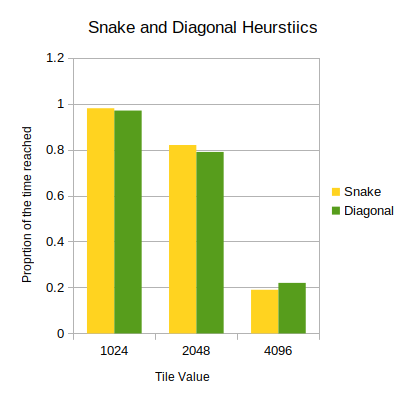
\includegraphics[width=0.4\textwidth]{SnakeToDiagonal.png}
    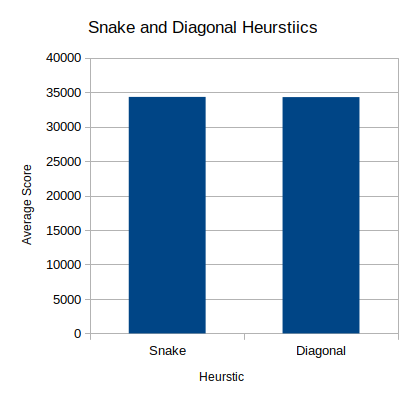
\includegraphics[width=0.4\textwidth]{SnakeToDiagonalScore.png}
    \caption{A compassion between the snake and the diagonal heuristics.}
    \label{fig:SnakeVDiagonal}
\end{figure}
\subsubsection{Compassion between Snake and Diagonal Heuristics}
After implementing these heuristics, the maximum tiles and scores were logged for 100 games using each heuristic. There was no statistically significant difference between the two heuristics, as shown in Figure \ref{fig:SnakeVDiagonal}.


\section{Dynamically Generating Heuristics for a n x m game}
Specific heuristics are easy to adapt to any size of the 2048 game, such as summing up all the cells in a grid; however, generating a weighted matrix for any game is much more difficult. Some heuristics do not have an obvious formula to generate the weights matrix. To start this process,  I made variable-sized but still square heuristics.
\subsection{Dynamic Snake}
As it leads to a simpler algorithm to generate the matrix, the smallest cell it at the top left, and the largest cell will be at the bottom corner (depending on the matrix size).
It can be generated using the following code. 
\begin{algorithm}
\caption{Dynamic Snake}\label{DynamicSnake} 
\begin{algorithmic}[1]
\Procedure{DynamicSnake}{row, col}
\State powers $\gets$ double[row][col]
\For {$i \gets 0$ to row$ - 1$}
\For {$j \gets 0$ to col$ - 1$}
\If {i \% 2 == 0}
\State $k \gets j$ 
\Else
\State $k \gets $row$ - j - 1$ 
\EndIf
\State power[$i$][$j$] $\gets 4^{i*col + k}$
\EndFor
\EndFor
\EndProcedure
\end{algorithmic}
\end{algorithm}
While the algorithm works on rectangular games, this heuristic is optimised for square games. A square game is more symmetrical than a rectangular game. There are eight theoretically equivalent rotations and reflections for a square game. In rectangular games, there would only be four rotations that would be more optimal. To determine which rotations were the best for different, the Dynamic Snake heuristic was run on several $n \times m$ and $m \times n$. In every pair, the heuristic performed better in the games which were wider than tall.

A solution is generating a matrix that goes up from the bottom right along the longer edge, depending on which way that is.

A few techniques were tried to improve the performance of the Dynamic Snake heuristic:
\subsubsection{Symmetrical Heuristic}
The snake heuristic is made by calculating a weighted sum, the current weighted matrix There are eight theoretically equivalent rotations of this matrix.
\[
\begin{matrix}
\text{Original} \\
\begin{bmatrix}
    2^{0} & 2^{1} & 2^{2} & 2^{3} \\
    2^{7} & 2^{6} & 2^{5} & 2^{4} \\
    2^{8} & 2^{9} & 2^{10} & 2^{11} \\
    2^{15} & 2^{14} & 2^{13} & 2^{12}
\end{bmatrix}
&
\begin{bmatrix}
    2^{3} & 2^{2} & 2^{1} & 2^{0} \\
    2^{4} & 2^{5} & 2^{6} & 2^{7} \\
    2^{11} & 2^{10} & 2^{9} & 2^{8} \\
    2^{12} & 2^{13} & 2^{14} & 2^{15}
\end{bmatrix}
&
\begin{bmatrix}
    2^{15} & 2^{14} & 2^{13} & 2^{12} \\
    2^{8} & 2^{9} & 2^{10} & 2^{11} \\
    2^{7} & 2^{6} & 2^{5} & 2^{4} \\
    2^{0} & 2^{1} & 2^{2} & 2^{3}
\end{bmatrix}
&
\begin{bmatrix}
    2^{12} & 2^{13} & 2^{14} & 2^{15} \\
    2^{11} & 2^{10} & 2^{9} & 2^{8} \\
    2^{4} & 2^{5} & 2^{6} & 2^{7} \\
    2^{3} & 2^{2} & 2^{1} & 2^{0}
\end{bmatrix}
\\

\\
\begin{bmatrix}
    2^{0} & 2^{7} & 2^{8} & 2^{15} \\
    2^{1} & 2^{6} & 2^{9} & 2^{14} \\
    2^{2} & 2^{5} & 2^{10} & 2^{13} \\
    2^{3} & 2^{4} & 2^{11} & 2^{12}
\end{bmatrix}
&
\begin{bmatrix}
    2^{15} & 2^{8} & 2^{7} & 2^{0} \\
    2^{14} & 2^{9} & 2^{6} & 2^{1} \\
    2^{13} & 2^{10} & 2^{5} & 2^{2} \\
    2^{12} & 2^{11} & 2^{4} & 2^{3}
\end{bmatrix}
&
\begin{bmatrix}
    2^{3} & 2^{4} & 2^{11} & 2^{12} \\
    2^{2} & 2^{5} & 2^{10} & 2^{13} \\
    2^{1} & 2^{6} & 2^{9} & 2^{14} \\
    2^{0} & 2^{7} & 2^{8} & 2^{15}
\end{bmatrix}
&
\begin{bmatrix}
    2^{12} & 2^{11} & 2^{4} & 2^{3} \\
    2^{13} & 2^{10} & 2^{5} & 2^{2} \\
    2^{14} & 2^{9} & 2^{6} & 2^{1} \\
    2^{15} & 2^{8} & 2^{7} & 2^{0}
\end{bmatrix}
\end{matrix}
\]
Usually, the dynamic snake heuristic is implemented using the first weight matrix, labelled original. The symmetrical version of a 2048 game would take the maximum weighted sum with all four matrices.

The results show a 
\subsubsection{Anti-trap}
From now on, the smallest weighted cell on the bottom row (bottom right in a $4 \times 4$ game) will be called the trap cell. The cell above the trap cell is only rewarded if its value is less than or equal to the value of the trap cell. This effect was more interesting than that of the Symmetrical change. The percentage of games reaching 8192 was slightly increased; however, smaller values were less likely to be reached, and the game no longer reached 2048 in every game.
\subsubsection{Fail Wrappers}
Fail Ratio is a second heuristic designed to be wrapped around a different heuristic. If the game loses in this state, it multiplies the heuristic score by a constant multiplier. It was run with rations -1 $\rightarrow$ 1 stepping with increments of 0.2. The best ratio was 0.8, which slightly increased the chance of achieving 8192 \ref{tab:dsfail}.

Fail Setter was a similar approach; this was made with the Monotonic  (see \ref{subsec:mono}). Initially, the 'fail setter' had this built-in to the heuristic if a game was at an end-of-the-game state, it would set the value to 0.6 When the fail ratio was created, this was separated out into a fail wrapper; some testing determined setting a value of -1000 was slightly more effective. 
\begin{table}
    \centering
\begin{tabular}{|c|c c c c c c|}
    \hline
    Tile Reached & 0.0 & 0.2 & 0.4 & 0.6 & 0.8 & 1.0  \\
    \hline
     4096 & 67.16\%&66.17\%&71.14\%&73.13\%&70.65\%&45.77\%\\
     8192 &3.48\%&1.49\%&5.97\%&9.45\%&5.97\%&0.50\%\\
     \hline
\end{tabular}
    \caption{Results for Dynamic Snake With Fail Ratio. Ratio 1 is the same as not using it. (Depth=6)}
    \label{tab:dsfail}
\end{table}

\subsection{Monotonic}
\label{subsec:mono}
The second heuristic was designed so that very few adoptions would be needed for rectangular games. It was based on the heuristic used by \cite{_16k2048ai}. There are several key features in this heuristic:
\begin{itemize}
    \item Values - on the outside edges are added up.
    \item Monotony - penalises states where rows/columns don\textquotesingle t increase in the same direction.
    \item Free Cells - rewards states with more free cells.
    \item Fail Setter - The values are set to a given value if the state loses; so far, the optimal value is -1000.
\end{itemize}
This heuristic also approximates a more effective version of the diagonal and has constantly scored the highest in most game states, including rectangular ones. It is flexible enough not to need modifications for specific game states.

There was one modification, which attempted to be more accurate to the original. This would mean each row could increase in different directions. For example:
\[
\begin{bmatrix}
    -&-&-\\
    2&4&8\\
    64&32&16\\
\end{bmatrix}
\]
In the original, it would be a relatively high-scoring game state (for monotony).
Despite the discrepancy between the original and my implementation, this over-site
turned out to be very important for the algorithm\textquotesingle s performance.

As the monotony of a game is forced into one direction 

Using the original approach, I could not get a score higher than 1024 regularly.

As the monotony is forced in one direction horizontally and one direction vertically, this heuristic could be seen as a more flexible variant of the diagonal heuristic. Unlike the snake heuristic, it turned out that the increased flexibility is a positive thing.
\subsection{Square Performance}
Now that the two new heuristics have been developed, it will be interesting to compare them to each other of various square game sizes. A third heuristic, the largest lower, will also be compared as a baseline. The comparisons will cover 2 × 2 to 4 × 4 for a depth of 4, 6 and 7. 5 × 5 will only be run at a depth of 4. 
\begin{table}
    \centering
    \begin{tabular}{|cc|ccc|}
    \hline
    Grid Size&Tiles Reached&LL&DS&Mon\\
    \hline
\multirow{3}{*}{2x2 D=4}&8&100&100&100\\
&16&94&87&92\\
&32&2&2&9\\
\hline
\multirow{4}{*}{3x3 D=4}&32&99&100&100\\
&64&94&97&100\\
&128&46&85&95\\
&256&1&24&40\\
\hline
\multirow{4}{*}{4x4 D=4}&512&99&98&99\\
&1024&54&91&87\\
&2048&2&72&50\\
&4096&0&9&1\\
\hline
\multirow{5}{*}{5x5 D=4}
&2048&100&97&99\\
&4096&100&80&98\\
&8192&81&62&87\\
&16384&21&32&73\\
&32768&0&5&27\\
\hline
\multirow{3}{*}{2x2 D=6}&8&98&97&96\\
&16&94&83&51\\
&32&9&8&7\\
\hline
\multirow{3}{*}{3x3 D=6}&64&99&99&100\\
&128&66&94&99\\
&256&15&57&68\\
&512&0&0&7\\
\hline
\multirow{3}{*}{4x4 D=6}&1024&94&100&99\\
&2048&34&95&90\\
&4096&0&73&57\\
&8192&0&9&5\\
\hline
\multirow{2}{*}{2x2 D=7}&16&95&92&93\\
&32&9&10&10\\
\hline
\multirow{3}{*}{3x3 D=7}&128&87&96&97\\
&256&33&63&84\\
&512&0&6&19\\
\hline
\multirow{5}{*}{4x4 D=7}&512&99&100&100\\
&1024&92&100&100\\
&2048&64&97&99\\
&4096&4&82&76\\
&8192&0&23&22\\
\hline
    \end{tabular}
    \caption{Square game performance}
    \label{tab:square}
\end{table}

On a depth of 6 2x2 (See table \ref{tab:square}, it very clearly performs best using the largest lower. Interestingly, the heuristics have evened out by the time we reach a depth of 7. I suspect that on a depth of 7, any reasonable heuristic will work for a 2x2 game. These games are very short, and all three heuristics are close to the maximum rate of achieving 32. In a 2 × 2 game, achieving 32 in more than 10\% on average is impossible. To get 32, you must first have a game state with a 16, 8 and 4 before a cell is added, e.g. $\big[\begin{smallmatrix}
  16 & 8\\
  4 & -
\end{smallmatrix}\big]$,
when a random cell is inserted, it must be a four. Otherwise, the game will end, which will only happen 10\% of the time. Very intriguingly, 2 × 2 Monotonic actually outperforms itself on depth 4, over depth 6. A similar situation occurs for the lower 2 × 2 Dynamic Snake values.

For the 3 × 3 games, the monotonic heuristic is the strongest by a long lead for depths 4, 6 and 7. Monotonic is often the most effective heuristic across the results in Tables \ref{tab:square} and \ref{tab:LLLR}, showing that his heuristic is very flexible. On the other hand, Dynamic-Snake is the most effective only for 4 × 4 games of depth 4 and 6. This suggests Dynamic Snake has optimised very effectively for lower depth 4 × 4 games; however, as the algorithm is more efficient, its usefulness reduces.
In 4 x 4 games, we can see that at depths of 4, the dynamic snake heuristic significantly outperforms. It is possible that changing the powers in the heuristic could yield different results. However, this is likely because the snake heuristic enforces a human strategy. This is very effective for humans as keeping track of everything that could happen in the next few moves is challenging. Following a strategy makes it easy to minimise the risk without looking further ahead. Past a certain point, a more flexible heuristic allows for good moves a human may struggle to see. For example, when using the Monotonic heuristic is quite common for the algorithm to switch the corner the greatest value is in. This is a sequence of moves where a human player may not risk it, as it is difficult to imagine the side effects. Similarly, the Dynamic Snake heuristic is effective on lower depths as it can minimise the risk; however, on deeper searches, the risk can be minimised more effectively by the expectimax algorithm.  

\subsection{Rectangular Performance}
There are several factors to investigate here to determine the best heuristic and adaptions for each. An adaption of a heuristic made early, Largest Lower, on a test was used to get a baseline performance for each shape. To accompany this heuristic, a Largest Right heuristic was also made. They are equivalent to a weighted sum for each of these matrices (Given a $n \times m$ game).
$$
\begin{matrix}
    \begin{bmatrix}
        1 & \hdots & 1 \\
        2 & \hdots & 2 \\
        \vdots & \hdots & \vdots \\
        n & \hdots & n
    \end{bmatrix}
    &
        \begin{bmatrix}
        1 & 2 & \hdots & m\\
        \vdots & \vdots & \vdots  &\vdots\\
        1 & 2 & \hdots & m
    \end{bmatrix}
    \\
    \text{Largest Lower}&\text{Largest Right}
\end{matrix}
$$

The first job was to determine if there was a rule for which of these two heuristics performed the best on a variety of different-sized games. The games were chosen for having or being close to having 16 squares. This meant the theoretical maximums were relatively similar, and the decision trees would not be much larger than a topical 4x4 game. The sizes chosen were 2 × 9, 3 × 6 and 4 × 5; each game was played with a depth of 6.
\begin{table}
    \centering
\begin{tabular}{|c|cccccc|}
\hline
&LL 2x9&LR 2x9&LL 3x6&LR 3x6&LL 4x5&LR 4x5\\
\hline
256&95&100&100&100&100&100\\
512&57&100&99&100&100&100\\
1024&16&98&94&100&100&100\\
2048&0&84&46&99&98&100\\
4096&0&52&2&87&63&89\\
8192&0&11&0&35&10&36\\
\hline
&DS 2x9&DS 9x2&DS 3x6&DS 6x3&DS 4x5&DS 5x4\\
\hline
128&99&91&100&99&100&100\\
256&83&63&100&99&100&100\\
512&42&17&100&95&100&100\\
1024&3&1&99&78&99&100\\
2048&0&0&83&39&99&99\\
4096&0&0&34&3&95&95\\
8192&0&0&0&0&83&72\\
16384&0&0&0&0&24&3\\
\hline
&\multicolumn{2}{c}{Mon 2x9}&\multicolumn{2}{c}{Mon 3x6}&\multicolumn{2}{c|}{Mon 4x5}\\
\hline
512&\multicolumn{2}{c}{94}&\multicolumn{2}{c}{100}&\multicolumn{2}{c|}{100}\\
1024&\multicolumn{2}{c}{88}&\multicolumn{2}{c}{99}&\multicolumn{2}{c|}{100}\\
2048&\multicolumn{2}{c}{59}&\multicolumn{2}{c}{90}&\multicolumn{2}{c|}{100}\\
4096&\multicolumn{2}{c}{16}&\multicolumn{2}{c}{74}&\multicolumn{2}{c|}{99}\\
8192&\multicolumn{2}{c}{0}&\multicolumn{2}{c}{17}&\multicolumn{2}{c|}{77}\\
16384&\multicolumn{2}{c}{0}&\multicolumn{2}{c}{0}&\multicolumn{2}{c|}{26}\\
32768&\multicolumn{2}{c}{0}&\multicolumn{2}{c}{0}&\multicolumn{2}{c|}{2}\\
\hline
\end{tabular}
    \caption{Tile frequencies for each heuristic and size (\textbf{L}argst \textbf{L}ower,  \textbf{L}argest \textbf{R}ight and \textbf{D}ynamic \textbf{S}nake and \textbf{Mon}otonic)}
    \label{tab:LLLR}
\end{table}
The data in table \ref{tab:LLLR} shows that the more extreme the ratio, the more beneficial the Largest Right  over the Largest Lower. For example, on the 2 × 9 game LR can achieve 8192 11\% of the time while LL can only achieve 1024 16\% of the time. Meanwhile, while on the much square game, 5 × 4 can achieve 8192 with some consistency. These trends can only be applied to ratios that are wider than tall, however, it seems likely that the largest lower would work better on games that are taller than wide. More generally, this data suggests that when using a heuristic that weights tiles in a specific direction, it is best 

The dynamic snake has two distinct rotations in a rectangular matrix; for example in a 2 × 9 game, they may look like this:
$$
\begin{matrix}
    \begin{bmatrix}
        2^0 & 2^1 & 2^2 & 2^3 & 2^4 & 2^5 & 2^6 & 2^7 & 2^8 \\
        2^{17} & 2^{16} & 2^{15} & 2^{14} & 2^{13} & 2^{12} & 2^{11} & 2^{10} & 2^9 \\
    \end{bmatrix}  &
    \begin{bmatrix}
        2^0 & 2^3 & 2^4 & 2^7 & 2^8 & 2^{11} & 2^{12} & 2^{15} & 2^{16} \\
        2^1 & 2^2 & 2^5 & 2^6 & 2^9 & 2^{10} & 2^{13} & 2^{14} & 2^{17} \\
    \end{bmatrix} \\
    W_1 & W_2
\end{matrix}
$$
$W_1$ is already generated when a new instance of DynamicSnake is created. However, there is currently no way of creating $W_2$. A workaround for this is transposing the game instead of the heuristic.

A 2 × 9 using the heuristic $W_2$ should be comparable to a 9 × 2 game using $W_1$. Instead of implementing a way to generate $W_2$, I deiced to take advantage of this.

Using Dynamic Snake, I found that, in general, Dynamic Snake is not the ideal heuristic for fewer square grids (table \ref{tab:LLLR}). The best DS for each size only beats the best of LL and LR in one case, 4 × 5, which is almost square. The data seems to suggest that it is best for the Snake to zig-zag along the longer dimension.  It would be relatively simple to make the DS heuristic generate the optimal of the two matrices, however, this has not been implemented, as DS is never the best of the heuristics.

Finally, how does Monotonic compare to the three heuristics? There were no obvious adaptions for this heuristic (Table \ref{tab:LLLR}. For both 2 × 9 and 3 × 6 Monotonic is the second-best heuristic, only being beaten by LR, while for the more square game, 4 × 5 Monotonic is the best heuristic, having even scored 32k.

\label{sec:complexity}
\section{Complexity}
\label{subsec:time_comp}
\subsection{4 x 4 Game}
As the most effective heuristics are currently locked into a $4\times4$ game, I will calculate the time complexity when run on a $4 \times 4$ game, where $n$ is the maximum depth of the tree.

After each maximising node, the tree grows by at most 4. One for each possible move up, down, left and right.

A game starts with two cells; hypothetically, let\textquotesingle s say:

\[
\begin{bmatrix}
    2&2&-&-\\
    -&-&-&-\\
    -&-&-&-\\
    -&-&-&-\\
\end{bmatrix}
\]
The best case outcome is that these two cells are merged:
\[
\begin{bmatrix}
    4&-&-&-\\
    -&-&-&-\\
    -&-&-&-\\
    -&-&-&-\\
\end{bmatrix}
\]
This leaves 15 free cells for the new cell to appear; after this, there will be two cells again.
Therefore there can never be more than $15$ free cells.

Therefore the most children a chance node can have is $15\times2=30$.



Each node has constant time work, so the leaf nodes dominate the tree.



For every two layers, the number of leaf nodes multiplies at most $120$, and there are $n$ layers in the tree. Therefore their are $120^\frac n 2$ leaf nodes
$\therefore$ time complexity to calculate the next move is $120^\frac n 2 = O(\sqrt{120}^n) \approx O(10.954^n)$

\subsection{m x n Game}
Consider calculating the children of a max node: each max node has at most 4 children. The next state is calculated using Appendix \ref{subsec:movtil}.


$\Rightarrow$ For directions UP and DOWN, the time complexity of the move operation is $O(m^2n)$ and for LEFT and RIGHT the time complexity is $O(mn^2)$

$\Rightarrow$ calculating the children of the max node has time complexity $2O(mn^2) + 2O(m^2n)$.

Consider calculating the children of a chance node:

A grid has at least one nonzero tile $\therefore$ There are $mn - 1$ cases to consider.

\begin{figure}
    \centering
    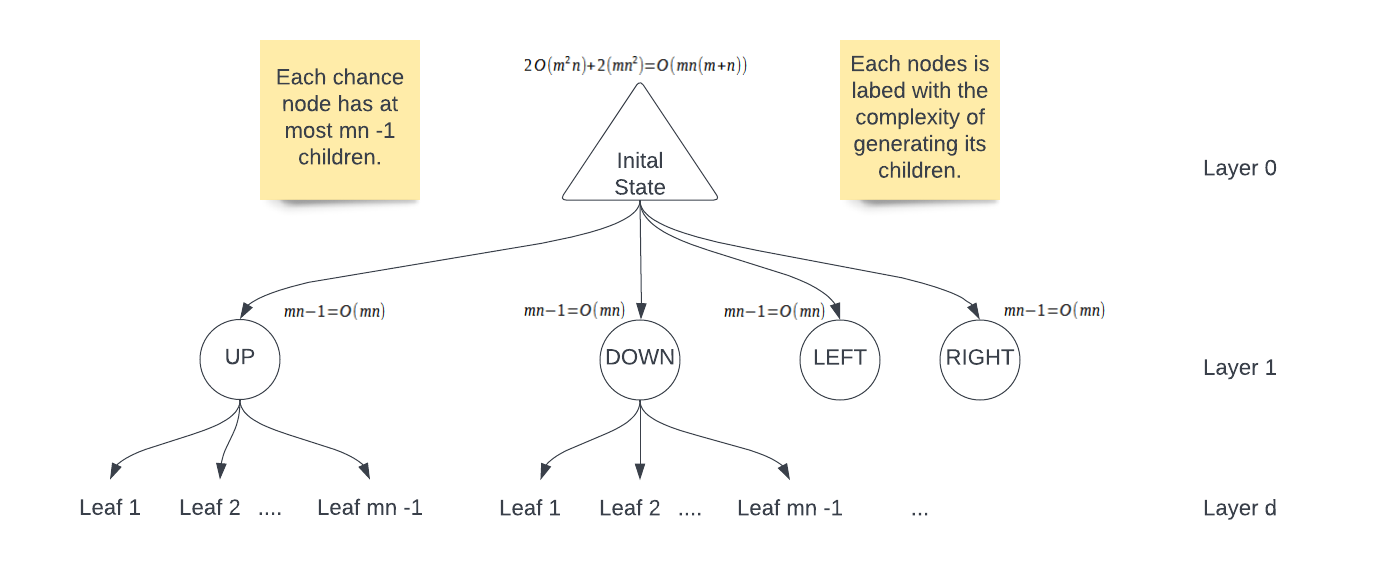
\includegraphics[width=0.8\textwidth]{expectimax tree.png}
    \caption{A tree for a n x m 2048 game}
    \label{fig:nm2048}
\end{figure}

By looking at Figure \ref{fig:nm2048}, it can be deduced that the number of work increases after every pair of layers, and the amount of work done generate the last two layers $d - 1$ and $d$ is: 

\begin{align}
\text{Time Complexity} & = 4^\frac{d}{2}(mn - 1)^{\frac{d - 2}{2}}O(mn(m+n)) + 4^\frac{d}{2}(mn - 1)^{\frac{d}{2}}O(mn)) \\
 & = O(4^\frac{d}{2}(mn - 1)^\frac{d - 2}{2}mn(m+n) + 4^\frac{d}{2}(mn - 1)^\frac{d}{2}mn) \\
 & = O(4^\frac{d}{2}(mn - 1)^\frac{d - 2}{2}mn(m + n + \underline{mn} - 1) \\
 & = O(4^\frac{d}{2}(mn - 1)^\frac{d}{2}m^2n^2)
\end{align}

When scoring the tree, all nodes, apart from the leaf nodes, are constant time, the leaf nodes are $O(nm) \therefore$, scoring the tree is $O(4^\frac{d}{2}(mn - 1)^\frac{d}{2}nm)$.
The term for generating the tree is still more significant, so the time complexity $= O(4^\frac{d}{2}(mn - 1)^\frac{d}{2}m^2n^2)$.

\newpage
\section{Optimisations}  
\subsection{Multi-threading}
Simple multi-threading is relatively easy to implement, in theory. Node children are independent of each other so that each child can be processed in a different thread. For example, when processing \ref{fig:threadtree}, you would start by generating the children of the root node; once these are generated, you would start four threads, one processing nodes A, B, C and D. The thread representing the root node would be set to inactive while waiting for the child threads to finish processing. Each child thread will generate its children and produce two threads for each node. A, B, C and D would be inactive until their children are calculated. There would be at most eight active threads simultaneously for this small example. The tree (depth=7) contains over 4 million leaf nodes for the game with the grid below.
$$
\begin{bmatrix}
     0 &0 &0 &0 \\2 &0 &0 &0 \\0 &0 &0 &2 \\0 &0 &0 &0
\end{bmatrix}
$$
This would lead to the maximum amount of threads at one time is four million.

While this is relatively simple, there are some series inefficiencies, partially in the number of threads created. Creating four million threads uses a lot of memory and stresses the scheduling algorithm, so another approach is needed. The solution is only to run a small number of threads from the tree. Ideally, a purpose-built system would be used to process the tree in a given number of threads; however, this would have been a very time-consuming process. Java has a feature called Parallel Streams \cite{pstreams} that can process an entire tree with the number of threads available on the system.

If processing the tree in figure \ref{fig:threadtree} using parallel java streams on a dual-core system (assuming the time each node is processed is identical) instead of the execution order of (Root), (A, B, C, D), (A1, A2, B1, B2, C1, C2, D1, D2) the new executive order would be (Root), (A, B), (A1, A2, B1, B2), (C, D), (C1, C2, D1, D2). This still leads to too many threads being generated at some stages of the tree; however, it is no longer a serious issue. The ideal solution would be creating a scheduling class to allocate tasks to a set number of threads on the same dual-core system; the previous example may look like this: (A, B), (A1, A2), (B1, B2), (C, D), (C1, C2), (D1, D2).
\begin{figure}
    \centering
    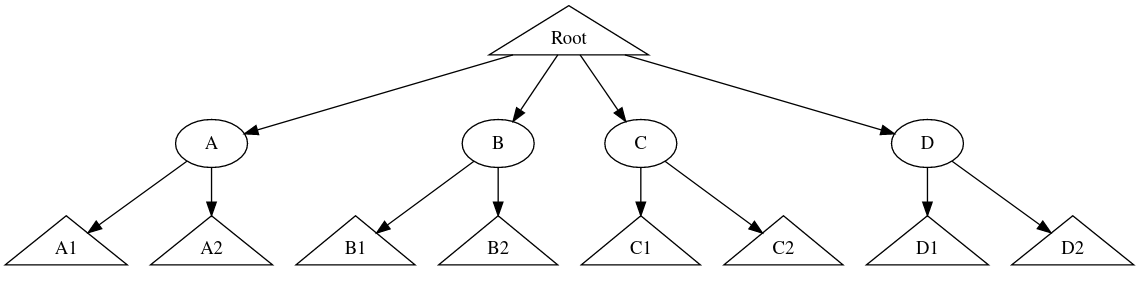
\includegraphics[width=0.8\textwidth]{tree.png}
    \caption{Example Tree}
    \label{fig:threadtree}
\end{figure}

Before multi-threading, for a 4x4 game, a depth of 4 was the best depth that could be processed reasonably. After implementing a threading approach with parallel streams, it could now process trees with a depth of 7. It also pushed enough to be able to reach 8192 somewhat regularly.

\subsection{Pruning}
\label{subsec:Pruning}
Pruning a tree is when you remove a branch from a tree without processing it. When done well, pruning should not impact which moves are chosen and, in some cases, may not even change the scores for those moves. For this problem, we will have to settle for unlikely to impact the moves chosen. 

The approaches used will be pruning unlikely possibilities. Due to the weighting of the nodes, unlikely possibilities have very little impact on the overall score. If their possibilities are unlikely enough it seems improbable, they would have much impact on what move is chosen. 

The other approach is pruning relatively bad moves; if a move is not the best option, it will not impact the score. Using the expectimax algorithm, it is not straightforward to determine with 100\% certainty that a move is not the best without calculating it. However, an educated guess can be made about how good a move is relative to its siblings.

To help analyse this, a simple text format was made to help view the tree; an example of this format is included at Apendix \ref{subsec:apendixtfile}.

The '\#' at before each number notes that a number follows. The second from the last number notes the Heuristic value of a given state, and the final value represents the derived or calculated score. Finally, the letter C, M or L represents if the node is a chance node, maximising node or leaf node. The number of space characters at the beginning of the line represents how deep it is in the tree. A small tool was written in C, using the library ncurses, to view these files in a collapsible form quickly.
\begin{figure}
    \centering
    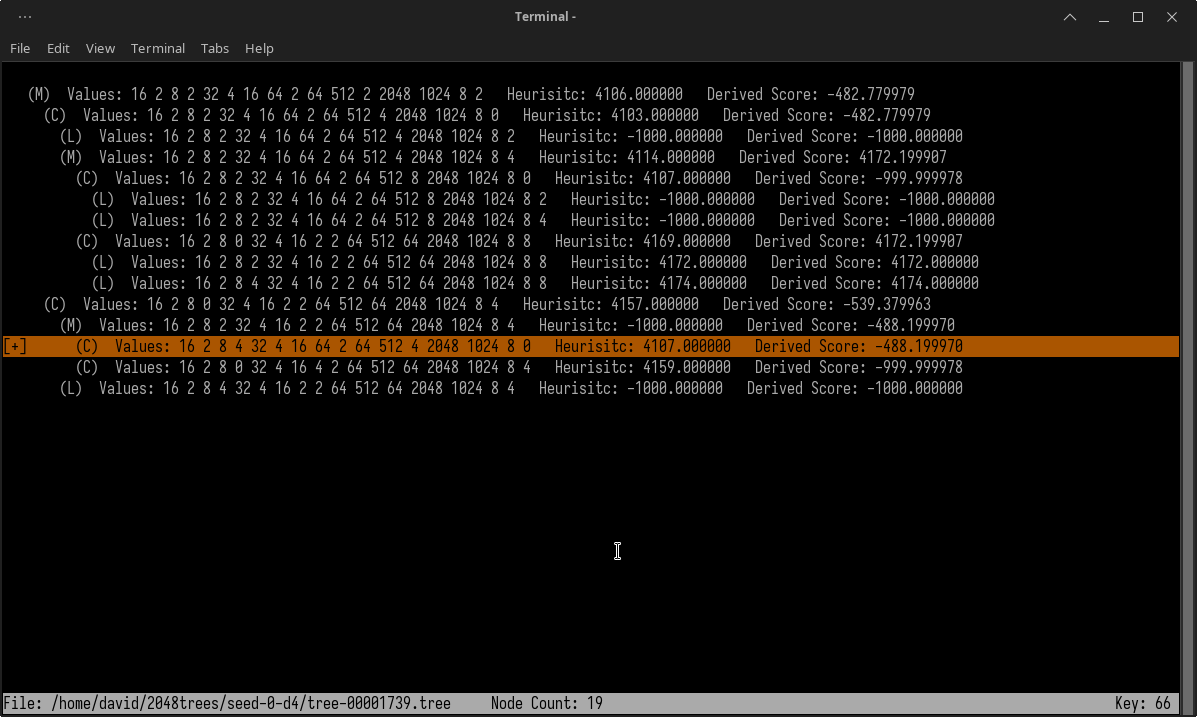
\includegraphics[width=1\textwidth]{Screenshot_2023-03-22_03-21-57.png}
    \caption{Tree View Tool}
    \label{fig:my_label}
\end{figure}
\subsubsection{Pruning Unlikely Possibilities}
\begin{figure}
    \centering
    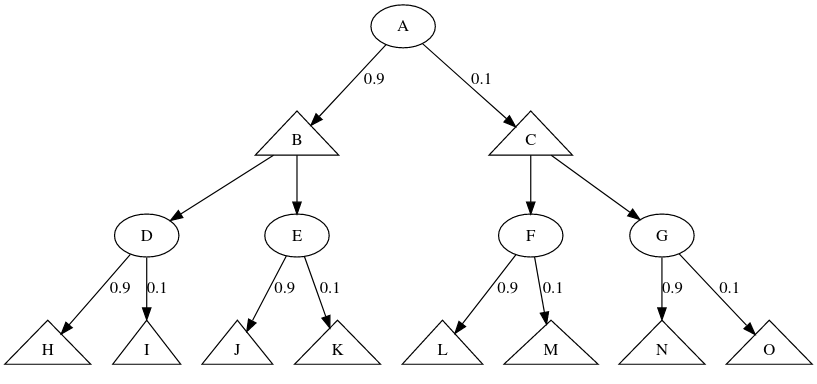
\includegraphics[width=1\textwidth]{unlikleypruning.png}
    \caption{Caption}
    \label{fig:unlikley}
\end{figure}
This approach is the simplest of the three in this section. It works by pruning unlikely possibilities. For example, if we take Figure \ref{fig:unlikley}, assume that the tree continues bellow nodes H - O. The nodes. For each respective move, there is only a 1\% chance of their $M$ or $O$ occurring. These nodes can be removed entirely from the tree.

Due to how my algorithm works internally, it is easier to prune all the children of a node rather simply pruning the node itself; however, due to the low weighting involved with these nodes, this show has very little impact on the final result. Determining which nodes to prune was quite a simple job. When generating an expetimax tree, a new parameter $count4$ (See Appendix \ref{subsec:apendixmulti}). When nodes and children are generated, and the node adds a four to the game, the value of $count4$ is decremented before being passed to the children. If the value of $count4$ is 0, the children will not be generated.

\begin{table}[]
    \centering
    \begin{tabular}{|c|ccc|}
    \hline
Tile Reached&No Pruning&3&2\\
\hline
1024&100&100&100\\
2048&99&99&99\\
4096&76&86&76\\
8192&22&24&14\\
\hline
Median Time&11m21.390s&8m15895ms&6m23.285s\\
Improvement&&1.37&1.78\\
\hline
    \end{tabular}
    \caption{Pruning (Monotonic /w FailSetter, d=7)}
    \label{tab:pruning}
\end{table}

The results were somewhat surprising for this. At least for the settings chosen, it turned out that pruning after seeing three 4s had a gain in both time and results. Even pruning after seeing two 4s only offered an 8\% reduction in the number of 8192 achieved and yet completed 1.78x faster. It is possible the increase in results may have be because the algorithm unlikely extremes are being pruned from the tree. If there is an unlikely but very rewarding or penalised state being pruned. This would mean that the unlikely extremes would be ignored, when they later don't happen the algorithm hasn't taken them into account.

\subsubsection{Pruning Poor Moves}
The first difficulty here is defining what a poor move is; there are two definitions below:
\begin{itemize}
    \item Moves which score a significantly lower heuristic than parent nodes even after a few moves.
    \item Moves that are currently scoring worse than already calculated siblings.
\end{itemize}

While both of these approaches seem straightforward, they have their complexities; due to time constraints, neither approach has yet been implemented.

A threshold value is needed to determine how unlikely a node must be before it is pruned.

The approach is easy when using multi-threading to help calculate the tree. However, it could be problematic when there are only poor moves. It is not difficult to imagine a situation where the game instead gives up because no moves meet the threshold for a good move. Ensuring it does not prune the best move on a specific branch is challenging.

A solution to this would be comparing nodes to their siblings; we can say with much more certainty if we are pruning moves that are likely worse than their siblings.

For example, using the tree in figure \ref{fig:prunepmoves}, if we assume that the nodes D, E, F and G all contain large sub-trees that are not shown. We would calculate node B's score as 100, as the average of D and E is 100; next, we would begin calculating C. With F having a score of 1, $x \ge 199$. While it is possible, it seems unlikely that $x \ge 199 \times v(F)$. The exact number we can say where this is unlikely would likely vary by the heuristic. For example, using the sum cells heuristic, you would expect the siblings of a chance node to be quite similar, as there is no weighting. However, a strongly weighted heuristic like Snake can see significant changes from rearranging tiles.

There is one large floor with this approach for this current project, which is multi-threading will no longer be straightforward. The child branches are no longer independent from each other.

While I don\textquotesingle t have data supporting this, I suspect that Pruning based on the scores of the siblings would be the most effective approach for pruning the tree out of the three discussed here. It would be interesting to compare the benefits of this pruning to multi-threading.

\begin{landscape}
    \begin{figure}
    \centering
    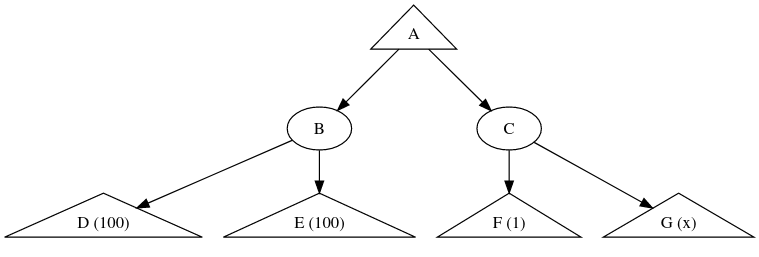
\includegraphics[width=1.5\textwidth]{pruningExample.png}
    \caption{An expectimax tree which can be pruned.}
    \label{fig:prunepmoves}
\end{figure}
\end{landscape}




\begin{landscape}
\begin{figure}
    \centering
    \includegraphics[width=1.30\textwidth]{dynamic_depth.png}
    \caption{Graph of Number of L5 Nodes to depth (4x4 game)}
    \label{fig:dynamic_depth_graph}
\end{figure}
    \begin{figure}
    \centering
    \includegraphics[width=1.30\textwidth]{dynamic_depth_free_cells.png}
    \caption{Graph of Number of L5 Nodes to depth (4x4 game)}
    \label{fig:dynamic_depth_free_graph}
\end{figure}
\end{landscape}

\subsection{Dynamic Depth}
\label{subsec:dyndep}
There is a strong trend in the data that deeper searches achieve large tiles more frequently (table \ref{tab:depth}). This idea was inspired by \cite{expectimax2048}; this implementation of expectimax uses a depth of eight when if there are less than four empty tiles on the grid; otherwise, a depth of 6 is used. This is possible because there are fewer possible outcomes with more free cells.

\begin{table}
    \centering
    \begin{tabular}{|c| c c  cc | c |}
\hline
Tiles Reached&2&4&6&7&$d(x)^*$\\
\hline
256&92&100&100&100&100\\
512&60&99&100&100&100\\
1024&15&87&99&100&100\\
2048&0&50&90&99&100\\
4096&0&1&57&76&100\\
8192&0&0&5&22&80\textsc{**}\\
16384&0&0&0&0&10\\
\hline
Median Time & 40ms & 711.5ms & 1m23.259s & 11m22.593s & 1h15m52.420s\\
\hline
    \end{tabular}
    \caption{Tiles achieved by depth (4x4 Monotonic /w Fail Setter).  }
    \label{tab:depth}
    \par{\textsc{*}Tested on a sample size of 10 due to high processing time.}
    \par{\textsc{**} One game ran out of memory on 4096.}
\end{table}

When there are fewer free cells in the grid, the tree can be explored deeper. As the branching factor on the tree is lower. Creating a function $d(x)$ was a complex process. I started by including a simple feature in the program. When the program is started with the command line argument '-d', it can probe the tree to see how far be generated in a given period. Using a python script, I picked ten random game states with each of 0-14 free cells from a game I had saved to my laptop. I created a CSV file which contained the number of nodes in each layer of the tree, the number of free cells in the state and the maximum depth achieved in 3 seconds. The game states that more available cells didn't have ten samples to pick from some groups.

I created a tool in c, reusing some code from tree view (See Section \ref{subsec:Pruning}) to analyse the trees for these nodes reporting how many nodes there were in each tree layer.

When creating a depth function, it is important to ensure that it doesn't overestimate, if an overestimate is produced, the program will hang until it runs out of memory. \cite{expectimax2048} used an approach based on the number of free cells in the grid, however, while avoiding overestimates this would limit me to at most a depth of 10 (Figure \ref{fig:dynamic_depth_free_graph}). Despite what is shown on Figure \ref{fig:dynamic_depth_graph} it is possible to complete an entire 4 × 4 game of 2048 with a depth of 7. This means that after a move is made, there is a depth 5 expectimax tree already calculated. If we count the number of nodes at the 5th level of this tree, and call it $k$, we can use this as the predictor for how deep the tree can be generated (See Figure \ref{fig:dynamic_depth_graph}). The function $f(x)$ from figure \ref{fig:dynamic_depth_graph}, however, will regularly overestimate.

The first thing I tried using $h(x) = \text{max} (\text{floor}~f(x), 7)$. This function only worked well towards the upper end of depth 8, where it was prone to overestimating. I rewrote the function $f(x)$ in the format $f(x) = 21x^{-b} -c$ i.e. $f(x)$ i.e. $b\approx 0.113$ and $c = 0$, and plotted it. I gradually decreased the value of b and increased c.

Checking that $floor~f'(x)$ was less than or equal to each point in the scatter graph. I eventually settled on $f'(x)=21x^{-0.065} - 3.75$. As with the original $f(x)$, this new depth function was modified to $d(x) = \text{max}(\text{floor}~f'(x), 7)$
 
To increase the certain this function was valid I ran a test on a game with seed=0 using the Monotonic Heuristic, however, my testing was limited as the game took approximately 1h 30m to run. My results for death, 6, 7 and $d(x)$ are below.

\[
\begin{matrix}
\begin{bmatrix}
    2&8&4&2 \\
    4&16&64&16 \\
    2048&512&256&32\\ 
    4096&1024&16&128 
\end{bmatrix}&
\begin{bmatrix}
    8192&512&32&16 \\
    4096&256&64&8 \\
    1024&128&16&4 \\
    8&16&8&2 
\end{bmatrix}&
\begin{bmatrix}
    8192&4096&512&4\\
    2048&1024&64&16\\
    128&64&32&8\\
    8&2&4&2
\end{bmatrix}
\\
d=6&d=7&d=d(x)
\end{matrix}
\]
After this, the performance of the algorithm was benchmarked by running it on 10 different games (See Table \ref{tab:depth}). This showed that the function $d(x)$ was very effective, reaching at least $8192$ in $8$ games, and even getting 16k once. However, in one game the function produced an overestimate, this game was not completed and instead was abandoned with a max tile of 4096.

The other drawback of this approach is the great reduction of performance. When using a constant depth, a game normally takes a while to get started but towards the end, is becomes relatively easy to calculate the trees. When using Dynamic Depth your are not only maximising the results from an expetimimax implementation but maximising the time it takes on a problem.
\section{Professional Issues: Licensing}
\label{sec:prof_issues}
Licensing is relevant to this project as the game 2048's source code is available under the MIT Licence on GitHub \cite{source2048}. This is a very permissive licence, meaning there are few restrictions on how one can use the published work for \cite{osi_faq}. This allows for dubious ethical situations where a large company uses the code internally without publishing, paying for or even acknowledging the use of that code. Copyleft licenses were created to deal with this issue (see \ref{subsec:oss}).

\subsection{Open-source Software}
\label{subsec:oss}
Open-source software is any software released under a license considered to be open-source. These licenses allow the source to be "freely accessed, used, changed and shared (in modified or unmodified form) by anyone." \cite{osi_faq}.

There are two major categories of open-source licenses: copyleft and permissive licenses. 

A copyleft licence, such as the various versions of the GNU General Public License \cite{gnu_copyleft}. The main purpose of copyleft is to protect open-source software from being converted to or re-used in property software. Copyleft licenses tend to be more complex and difficult to understand; for example, GPLv3 is 674 lines, while the permissive MIT license only has 21 lines. Complex licences can lead to issues, such as licence incompatibility; for example, the CDDL license is widely considered to be incompatible with the GLP licence \cite{gnu_cddl}; this makes it difficult to use code from software from these two licenses in the same code-base, despite the similar intent of these two licences. The simplest definition of a permissive license is simply an open source licence that is not copylefted \cite{osi_faq}.

\subsection{Open source software in this project}
\label{subsubsec:ossinthis}
This project has benefited from various pieces of open software, more than is possible to credit. Some examples are:
\begin{multicols}{2}
\begin{samepage}
Environment:
\begin{itemize}
    \item OpenJDK (GPL-v2.0)
    \item Maven (Apache 2.0)
    \item Git (GPL-v2.0)
    \item Overleaf (AGPL-3.0)
    \item Intellij (Apache-2.0)
\end{itemize}
\end{samepage}
Refrences:
\begin{itemize}
    \item 2048 (MIT)
\end{itemize}
\columnbreak
\begin{samepage}
Video recording/editing software:
\begin{itemize}
    \item Kdenlive (GPLv3)
    \item OBS studio (GPL-2.0)
\end{itemize}
\end{samepage}
\begin{samepage}
Libraries:
\begin{itemize}
    \item JUnit Jupiter API (EPL 2.0)
    \item JavaFX (GPL-v2.0)
    \item Jackson Data format CSV (Apache 2.0)
\end{itemize}
\end{samepage}
\end{multicols}
Even though this project has massively benefited from the software listed above, there is no evidence of the Video recording/editor software or some of the software under the environment sections. It is not fair on these projects that they don't get the credit they deserve when they enable a task to be done well. For example, the video editor Kdenlive (Made by the KDE Team) was used to place the clips of the program running in the video with text and music. If the footage had just been recorded with OBS, the video would have been much longer and not as high quality.

Some of the source code used in the project is added from the original MIT 2048 code \cite{game2048}; however, being a permissive license, this imposes no restrictions on how the how can be used in the future. The other software listed above has only been used in the development or is required to run the software. For example, the code could be packaged into a binary and sold without mentioning the open-source software and  breaking licenses would not be broken. While legally, this behaviour would be considered acceptable, from an ethical perspective, this would be highly unethical as it would be profiting from another developer's work without even crediting that developer's work.

Currently, no source code has been used under a copyleft license in this project; however, if this were the case, a situation with a binary being sold would still be possible. The difference would be that the source code would have to be published under a compatible license and freely available. While it would still be profiting with the aid of another developer's code, other options do not involve paying for the software, such as compiling from a source or downloading a third-party binary from another source. For a well-researched user, the payment for a binary is a choice rather than the only way of using the software.

While the license does not require it, if this code were ever published, it would be worth putting a link to the 2048 GitHub page \cite{game2048} in the README file, as it was an inspiration to work on the project. Though this project \cite{game2048} has been described as the source code for 2048, however, in the README file, Gabriele Cirulli clearly states that the project is a clone of the Android app 1024 and Saming's 2048. While the source code for neither of these is public, and Saming's 2048 is no longer available, I have been incorrectly implying that Gabriele Cirulli created the concept of 2048.

\subsection{Unlicensed Source Code and Copyright}
Many publicly available, partially small, GitHub projects have never been licensed. In many of these situations, likely, the original developer does not object to people using their code, as they have been through the work of publishing it in the first place. Technically, using code from a project like this breaches the owner's copyright. GitHub makes it very easy to accidentally make the mistake of including unlicensed code or even basing an entire project on it. For example, even if the licence on a project does not allow for modification of the project, a fork button is displayed to the user. A fork can be created without the user even being warned.

The heuristic function, diagonal's (see \ref{subsubsec:diag} code is currently heavily based on the code from the unlicensed GitHub project 2048-Game-Using-Expectimax \cite{expectimax2048}, as the educational exception to copyright covers this project, this is not a problem. From an ethical perspective, as long as the code remains publicly available and isn't used commercially, there is unlikely to be an issue; however, it does leave the project vulnerable to copyright claims if it is published. To avoid the risk of copyright claims, either the unlicensed code must be removed from the project or permission must be obtained to use the code.
\section{Self Evaluation}
Overall, this project has gone quite well. I have achieved an algorithm that can consistently reach the higher end of what humans can achieve. Some decisions, I think, held this project back, many of which were made very early in the project. Given enough time it is able to achieve 16k, which is more than expected to be able to reach when starting this project. Even more, performance can likely be extracted with minor tweaks to how the code works. For example very little testing has been done with some of the constraints inside most of the heuristics. One could likely extract better results by changing some of the constants in the monotonic heuristic or subtly changing the weights in the Dynamic-Snake heuristic.

Despite not being what I expected, the Monotonic heuristic is also very flexible; it can achieve a reasonable score highly on all the size games it has been tested on. For many of those games, it is the most effective I have made. Sadly due to the lack of other research in different-sized 2048 games, there is very little to compare these results to; however, out of all the published expectimax 2048 solvers, I found only one was able to achieve beyond 8192. This one was able to acheive 32k \cite{_16k2048ai}.


If I were to make another attempt at this project, there are a few things I would change early on.
\begin{enumerate}
    \item Using Java - Java was chosen because it was the most appropriate language I am confident in, not because it was the best language for the job. A faster language such as C++ or Rust would have been more appropriate.
    \item The game is tied too closely to the algorithm. Early in the project, I decided that the next stage of the game would be obtained from the algorithm. This means the algorithm has to keep track of irrelevant data, such as the game score. There are many repeated 'states' in an expectimax tree; however, there are very few situations where the scores are the same. This decision made it awkward and inelegant when I attempted to implement a form of memorisation. The close nature of the algorithm and the game makes it possible for an algorithm to cheat. A chance node could theoretically maliciously pick the next state to maximise results.
    \item I would investigate the possibility of more efficient ways of storing a game board. For example, \cite{_16k2048ai} stores the game in a 64-bit integer. This brings in a lot of new options for bringing down the processing time in heuristics, making moves quickly modifying the grid. This is particularly true with grids at most 4 × 4, which can easily be stored in a single 64-bit integer.
\end{enumerate}
Despite these problems, this implementation has some strengths.
\begin{enumerate}
    \item The multi-threading is very effective at utilising a CPU'S available resources to maximise performance.
    \item The implementation is very flexible in certain areas. Adding a new heuristic can be done quickly, and setting up the code for dynamic depth was also easy. Adding a new tree-based algorithm such as mini-max could be done by adding a new Node Behaviour; minimising nodes would have to return the smallest scoring node when asked for their score but return a random node when asked for the next node. New views and even models could be added with almost no extra work.
\end{enumerate}
\newpage
\appendix
\section*{Apendix}
\section{Video}
\label{subsec:vid}
\par{Some footage of the program running has been recorded and uploaded to YouTube.}
\href{https://youtu.be/WisBoM4lkQQ}{https://youtu.be/WisBoM4lkQQ}
\section{Proof Of Concepts}
\subsection{Decision Tree}
\label{subsubsec:apendixdt}
\begin{minted}{java}
public class TreeNode {
    private final TreeNode[] children;
    private float score;

    // While nicer interface will be used a weight of 1 is the same as unweighted.
    private final float weight;


    // Create leaf node
    public TreeNode(float weight, float score) {
        this.children = new TreeNode[0];
        this.score = score;
        this.weight = weight;
    }

    // Create branch node
    public TreeNode(float weight, TreeNode... children) {
        this.children = children;
        this.weight = weight;
    }

    // Getters and setters not included
}
\end{minted}
\subsection{Expectimax}
\label{subsec:apendixexpecti}
\begin{minted}{java}
package ProofOfConcept.Expectimax;

import ProofOfConcept.DecisionTree.TreeNode;

public class ChanceNode extends TreeNode {
    public ChanceNode(float weight, TreeNode... children) {
        super(weight, children);
        float sum = 0f;

        for (int i = 0; i < children.length; i++) {
            sum += children[i].getWeightedScore();
        }

        this.setScore(sum / children.length);
    }
}

package ProofOfConcept.Expectimax;

import ProofOfConcept.DecisionTree.TreeNode;

public class MaxNode extends TreeNode {
    private TreeNode optimalChild;

    public MaxNode(float weight, TreeNode... children) {
        super(weight, children);
        this.calcScore();
    }

    private void calcScore() {
        int count = this.getChildCount();
        float max = Float.NEGATIVE_INFINITY;

        for (int i = 0; i < count; i++) {
            float childWeight = this.getChild(i).getWeightedScore();
            if (childWeight > max) {
                max = childWeight;
                this.optimalChild = this.getChild(i);
            }
        }
        this.setScore(max);
    }

    @Override
    public TreeNode getNextNode() {
        return this.optimalChild;
    }
}

\end{minted}

\subsection{2048 Game}
\label{subsec:apendix2048}
\begin{minted}{java}
package ProofOfConcept.Game2048;

import java.util.stream.IntStream;

public enum DirectionVect {
    UP(-1, 0), DOWN(1, 0), LEFT(0, -1), RIGHT(0, 1);

    private final int i;
    private final int j;
    DirectionVect(int i, int j) {
        this.i = i;
        this.j = j;
    }

    public int getI() {
        return i;
    }

    public int getJ() {
        return j;
    }

    public IntStream getVRange(int height) {
        return getStream(this == DOWN || this == UP, height);
    }


    public IntStream getHRange(int width) {
        return getStream(this == LEFT || this == RIGHT, width);
    }

    private IntStream getStream(boolean dirAxis, int max) {
        boolean reversed = this == DOWN || this == RIGHT;
        IntStream stream;

        if (dirAxis) {
            stream = IntStream.range(1, max);
            if (reversed) stream = stream.map(i -> max - i - 1);
        } else {
            stream = IntStream.range(0, max);
        }
        return stream;
    }
}

package ProofOfConcept.Game2048;

import java.awt.*;
import java.util.ArrayList;
import java.util.Arrays;
import java.util.List;
import java.util.Random;

public class Game2048 {
    private final int width;
    private final int height;
    private long score;
    private final Random rnd;
    private int[][] grid;

    public Game2048(int width, int height, Random rnd) {
        this.width = width;
        this.height = height;
        this.rnd = rnd;
    }

    /*
     * Starts a game with 2 random starting cells.
     * This function can be called again to restart a game.
     */
    public void init() {
        this.grid = new int[height][width];
        this.score = 0;
        addRndCell();
        addRndCell();
    }

    public void loadCustomGame(int[][] grid) {
        this.grid = grid;
    }

    /*
     * Populates random free cells in the grid with free cells.
     */
    public void addRndCell() {
        List<Point> freeCells = this.getFreeCells();
        int i = this.rnd.nextInt(freeCells.size());
        this.grid[freeCells.get(i).x][freeCells.get(i).y] = 
            this.rnd.nextFloat() > 0.9 ? 4 : 2;
    }

    private List<Point> getFreeCells() {
        List<Point> cells = new ArrayList<>(width * height);
        for (int i = 0; i < this.height; i++) {
            for (int j = 0; j < this.width; j++) {
                if (this.grid[i][j] == 0) {
                    cells.add(new Point(i, j));
                }
            }
        }
        return cells;
    }

    public boolean move(DirectionVect dir) {
        boolean[][] merged = new boolean[height][width];
        boolean flag = false;
        for (int i : dir.getVRange(this.height).toArray()) {
            for (int j : dir.getHRange(this.width).toArray()) {
                if (grid[i][j] != 0) {
                    if (moveCell(i, j, dir, merged)) {
                        flag = true;
                    }
                }
            }
        }
        return flag;
    }


    @Override
    public String toString() {
        return "Game2048{" + "width=" + width + ", height=" + height + ", grid=" + 
             Arrays.deepToString(grid) + '}';
    }

    private boolean moveCell(final int row, final int col, 
            DirectionVect dir, boolean[][] merged) {
        int i = row;
        int j = col;

        while (inGrid(i + dir.getI(), j + dir.getJ()) && 
               grid[i + dir.getI()][j + dir.getJ()] == 0) {
            i += dir.getI();
            j += dir.getJ();
        }

        if (inGrid(i + dir.getI(), j + dir.getJ()) && 
                grid[row][col] == grid[i + dir.getI()][j + dir.getJ()] && 
                !merged[i + dir.getI()][j + dir.getJ()]) {
            this.grid[i + dir.getI()][j + dir.getJ()] <<= 1;
            merged[i + dir.getI()][j + dir.getJ()] = true;
            this.grid[row][col] = 0;
            this.score += this.grid[i + dir.getI()][j + dir.getJ()];
            return true;
        } else if (!(i == row && j == col)) {
            this.grid[i][j] = this.grid[row][col];
            this.grid[row][col] = 0;
            return true;
        }
        return false;

    }

    private boolean inGrid(int i, int j) {
        return 0 <= i && i < this.height && 0 <= j && j < this.width;
    }

    public long getScore() {
        return score;
    }

    public void print() {
        for (int i = 0; i < height; i++) {
            for (int j = 0; j < width; j++) {
                System.out.printf("%5d", this.grid[i][j]);
            }
            System.out.println();
        }
    }
}

package ProofOfConcept.Game2048;

import java.util.Random;
import java.util.Scanner;

public class Driver {
    public static void main(String[] args) {
        Scanner scan = new Scanner(System.in);
        Random rnd = new Random();

        int w, h;
        w = scan.nextInt();
        h = scan.nextInt();

        Game2048 game2048 = new Game2048(w, h, rnd);
        game2048.init();

        while (true) {
            System.out.println(game2048.getScore());
            game2048.print();

            char i = scan.next("[wWaAsSdD]").charAt(0);

            switch (i) {
                case 'w', 'W' -> {
                    if (game2048.move(DirectionVect.UP)) game2048.addRndCell();
                }
                case 's', 'S' -> {
                    if (game2048.move(DirectionVect.DOWN)) game2048.addRndCell();
                }
                case 'a', 'A' -> {
                    if (game2048.move(DirectionVect.LEFT)) game2048.addRndCell();
                }
                case 'd', 'D' -> {
                    if (game2048.move(DirectionVect.RIGHT)) game2048.addRndCell();
                }
            }
        }
    }
}


\end{minted}
\subsection{2048 expectimax}
\label{subsec:apendixauto2048}
\begin{minted}{java}
package ProofOfConcept.Auto2048;

import ProofOfConcept.Game2048.DirectionVect;

import java.awt.*;
import java.util.ArrayList;
import java.util.Arrays;
import java.util.List;
import java.util.Random;

public abstract class Node2048 {
    protected float nodeScore;
    protected Random rnd;
    protected Node2048[] children;
    private final int width;
    private final int height;
    private long score;
    private int[][] grid;
    public Node2048() {
        this(new Random());
    }

    public Node2048(Random rnd) {
        this.width = 2;
        this.height = 2;
        this.rnd = rnd;
    }

    public int getWidth() {
        return width;
    }

    public int getHeight() {
        return height;
    }

    protected Node2048 cloneAs(Node2048 as) {
        as.grid = new int[this.height][this.width];
        as.score = this.score;
        as.rnd = rnd;

        for (int i = 0; i < this.height; i++) {
            System.arraycopy(this.grid[i], 0, as.grid[i], 0, this.width);
        }

        return as;
    }

    protected void setChildren(Node2048[] children) {
        this.children = children;
    }

    /*
     * Starts a game with 2 random starting cells.
     * This function can be called again to restart a game.
     */
    public void init() {
        this.grid = new int[height][width];
        this.score = 0;
        addRndCell();
        addRndCell();
    }

    public void loadCustomGame(int[][] grid) {
        this.grid = grid;
    }

    /*
     * Populates random free cells in the grid with free cells.
     */
    public void addRndCell() {
        List<Point> freeCells = this.getFreeCells();
        int i = this.rnd.nextInt(freeCells.size());
        this.grid[freeCells.get(i).x][freeCells.get(i).y] = this.rnd.nextFloat() > 0.9 ? 4 : 2;
    }

    public abstract Node2048[] expectimax();

    public List<Point> getFreeCells() {
        List<Point> cells = new ArrayList<>(width * height);
        for (int i = 0; i < this.height; i++) {
            for (int j = 0; j < this.width; j++) {
                if (this.grid[i][j] == 0) {
                    cells.add(new Point(i, j));
                }
            }
        }
        return cells;
    }

    public boolean move(DirectionVect dir) {
        boolean[][] merged = new boolean[height][width];
        boolean flag = false;
        for (int i : dir.getVRange(this.height).toArray()) {
            for (int j : dir.getHRange(this.width).toArray()) {
                if (grid[i][j] != 0) {
                    if (moveCell(i, j, dir, merged)) {
                        flag = true;
                    }
                }
            }
        }
        return flag;
    }


    @Override
    public String toString() {
        return Arrays.deepToString(grid);
    }

    private boolean moveCell(final int row, final int col, DirectionVect dir, boolean[][] merged) {

        int i = row;
        int j = col;

        while (inGrid(i + dir.getI(), j + dir.getJ()) && grid[i + dir.getI()][j + dir.getJ()] == 0) {
            i += dir.getI();
            j += dir.getJ();
        }

        if (inGrid(i + dir.getI(), j + dir.getJ()) && grid[row][col] == grid[i + dir.getI()][j + dir.getJ()] && !merged[i + dir.getI()][j + dir.getJ()]) {
            this.grid[i + dir.getI()][j + dir.getJ()] <<= 1;
            merged[i + dir.getI()][j + dir.getJ()] = true;
            this.grid[row][col] = 0;
            this.score += this.grid[i + dir.getI()][j + dir.getJ()];
            return true;
        } else if (!(i == row && j == col)) {
            this.grid[i][j] = this.grid[row][col];
            this.grid[row][col] = 0;
            return true;
        }
        return false;

    }

    private boolean inGrid(int i, int j) {
        return 0 <= i && i < this.height && 0 <= j && j < this.width;
    }

    public long getScore() {
        return score;
    }

    public void print() {
        for (int i = 0; i < height; i++) {
            for (int j = 0; j < width; j++) {
                System.out.printf("%5d", this.grid[i][j]);
            }
            System.out.println();
        }
    }

    protected void setCellValue(int i, int j, int val) {
        this.grid[i][j] = val;
    }

    public abstract Node2048 nextNode();


    public float heuristic() {
        float sum = 0f;
        for (int i = 0; i < this.getHeight(); i++) {
            for (int j = 0; j < this.getWidth(); j++) {
                sum += this.grid[i][j];
            }
        }

        return sum;
    }
}

package ProofOfConcept.Auto2048;

import java.awt.*;
import java.util.ArrayList;
import java.util.List;

public class ChanceNode extends Node2048 {

    @Override
    public Node2048[] expectimax() {
        List<Point> cells = this.getFreeCells();
        List<Node2048> children = new ArrayList<>(cells.size() * 2);
        for (Point cell : cells) {
            Node2048 child1 = this.cloneAs(new MoveNode());

            child1.setCellValue(cell.x, cell.y, 2);

            children.add(child1);
        }
        Node2048[] nodes = children.toArray(new Node2048[0]);


        this.setChildren(nodes);

        this.nodeScore = 0;

        for (Node2048 node : nodes) {
            node.expectimax();
            this.nodeScore += node.nodeScore;
        }

        if (nodes.length > 0) {
            this.nodeScore /= nodes.length;
        } else {
            this.nodeScore = getScore();
        }

        return nodes;
    }

    @Override
    public Node2048 nextNode() {
        if (children.length > 0) {
            int next = rnd.nextInt(this.children.length);
            return this.children[next];
        } else {
            return null;
        }
    }
}


package ProofOfConcept.Auto2048;

import java.awt.*;
import java.util.ArrayList;
import java.util.List;

public class ChanceNode extends Node2048 {

    @Override
    public Node2048[] expectimax() {
        List<Point> cells = this.getFreeCells();
        List<Node2048> children = new ArrayList<>(cells.size() * 2);
        for (Point cell : cells) {
            Node2048 child1 = this.cloneAs(new MoveNode());

            child1.setCellValue(cell.x, cell.y, 2);

            children.add(child1);
        }
        Node2048[] nodes = children.toArray(new Node2048[0]);


        this.setChildren(nodes);

        this.nodeScore = 0;

        for (Node2048 node : nodes) {
            node.expectimax();
            this.nodeScore += node.nodeScore;
        }

        if (nodes.length > 0) {
            this.nodeScore /= nodes.length;
        } else {
            this.nodeScore = getScore();
        }

        return nodes;
    }

    @Override
    public Node2048 nextNode() {
        if (children.length > 0) {
            int next = rnd.nextInt(this.children.length);
            return this.children[next];
        } else {
            return null;
        }
    }
}


package ProofOfConcept.Auto2048;

import ProofOfConcept.Game2048.DirectionVect;

import java.util.ArrayList;
import java.util.List;

public class MoveNode extends Node2048 {
    Node2048 nextNodeI = null;

    @Override
    public Node2048[] expectimax() {
        List<Node2048> moves = new ArrayList<>(4);
        for (DirectionVect dir : DirectionVect.values()) {
            Node2048 child = this.cloneAs(new ChanceNode());

            if (child.move(dir)) moves.add(child);

        }

        Node2048[] nodes = moves.toArray(new Node2048[0]);
        this.setChildren(nodes);

        this.nodeScore = Float.NEGATIVE_INFINITY;

        for (Node2048 node : nodes) {
            node.expectimax();
            if (node.nodeScore > this.nodeScore) {
                this.nextNodeI = node;
                this.nodeScore = node.nodeScore;
            }
        }

        if (nodes.length == 0) {
            this.nodeScore = getScore();
        }

        return nodes;
    }

    @Override
    public Node2048 nextNode() {
        return this.nextNodeI;
    }
}


package ProofOfConcept.Auto2048;

public class Driver {
    public static void main(String[] args) {
        Node2048 root = new MoveNode();
        root.init();
        root.expectimax();

        while (root != null) {
            System.out.printf("Score : %d\n", root.getScore());
            root.print();
            root = root.nextNode();
        }
    }
}
\end{minted}

\subsection{2048 Heuristic}
\label{subsec:apendix2048H}
\begin{minted}{java}
package ProofOfConcept.Heuristic2048;

import ProofOfConcept.Game2048.DirectionVect;

import java.awt.*;
import java.util.ArrayList;
import java.util.Arrays;
import java.util.List;
import java.util.Random;

public abstract class Node2048
{
    public int getWidth()
    {
        return width;
    }

    public int getHeight()
    {
        return height;
    }

    protected float nodeScore;
    private int width;
    private int height;
    private long score;
    protected Random rnd;
    private int[][] grid;

    protected Node2048[] children;

    public Node2048()
    {
        this(new Random());
    }

    public Node2048(Random rnd)
    {
        this.width = 4;
        this.height = 4;
        this.rnd = rnd;
    }

    protected Node2048 cloneAs(Node2048 as)
    {
        as.grid = new int[this.height][this.width];
        as.score = this.score;
        as.rnd = rnd;

        for (int i = 0; i < this.height; i++)
        {
            for (int j = 0; j < this.width; j++)
            {
                as.grid[i][j] = this.grid[i][j];
            }
        }

        return as;
    }

    protected void setChildren(Node2048[] children)
    {
        this.children = children;
    }

    /*
     * Starts a game with 2 random starting cells.
     * This function can be called again to restart a game.
     */
    public void init()
    {
        this.grid = new int[height][width];
        this.score = 0;
        addRndCell();
        addRndCell();
    }

    public void loadCustomGame(int[][] grid)
    {
        this.grid = grid;
    }

    /*
     * Populates random free cells in the grid with free cells.
     */
    public void addRndCell()
    {
        List<Point> freeCells = this.getFreeCells();
        int i = this.rnd.nextInt(freeCells.size());
        this.grid[freeCells.get(i).x][freeCells.get(i).y] = this.rnd.nextFloat() > 0.9 ? 4 : 2;
    }

    public abstract void expectimax(int maxDepth);

    public List<Point> getFreeCells()
    {
        List<Point> cells = new ArrayList<>(width*height);
        for (int i = 0; i < this.height; i++)
        {
            for (int j = 0; j < this.width; j++)
            {
                if (this.grid[i][j] == 0)
                {
                    cells.add(new Point(i, j));
                }
            }
        }
        return cells;
    }

    public boolean move(DirectionVect dir)
    {
        boolean[][] merged = new boolean[height][width];
        boolean flag = false;
        for (int i: dir.getVRange(this.height).toArray())
        {
            for (int j: dir.getHRange(this.width).toArray())
            {
                if (grid[i][j] != 0)
                {
                    if (moveCell(i, j, dir, merged))
                    {
                        flag = true;
                    }
                }
            }
        }
        return flag;
    }


    @Override
    public String  toString()
    {
        return Arrays.deepToString(grid);
    }

    private boolean  moveCell(final int row, final int col, DirectionVect dir, boolean[][] merged)
    {

        int i = row; int j = col;

        while(inGrid(i + dir.getI(), j + dir.getJ()) &&
                grid[i + dir.getI()][j + dir.getJ()] == 0)
        {
            i += dir.getI();
            j += dir.getJ();
        }

        if (inGrid(i + dir.getI(), j + dir.getJ()) &&
                grid[row][col] == grid[i + dir.getI()][j + dir.getJ()] &&
                !merged[i + dir.getI()][j + dir.getJ()])
        {
            this.grid[i + dir.getI()][j + dir.getJ()] <<= 1;
            merged[i + dir.getI()][j + dir.getJ()] = true;
            this.grid[row][col] = 0;
            this.score += this.grid[i + dir.getI()][j + dir.getJ()];
            return true;
        }
        else if (!(i == row && j == col))
        {
            this.grid[i][j] = this.grid[row][col];
            this.grid[row][col] = 0;
            return true;
        }
        return false;

    }

    private boolean inGrid(int i, int j)
    {
        return 0 <= i && i < this.height && 0 <= j && j < this.width;
    }

    public long getScore()
    {
        return score;
    }

    public void print()
    {
        for (int i = 0; i < height; i++)
        {
            for (int j = 0; j < width; j++)
            {
                System.out.printf("%5d", this.grid[i][j]);
            }
            System.out.println();
        }
    }

    protected void setCellValue(int i, int j, int val)
    {
        this.grid[i][j] = val;
    }

    public abstract Node2048 nextNode();

    public float heuristic()
    {
        float score = 0;
        for (int i = 0; i < this.getHeight(); i++)
        {
            for (int j = 0; j < this.getWidth(); j++)
            {
                score += grid[i][j] * i;
            }
        }

        return score;
    }
}

package ProofOfConcept.Heuristic2048;

import java.awt.*;
import java.util.ArrayList;
import java.util.List;

public class ChanceNode extends Node2048 {

    @Override
    public void expectimax(int maxDepth) {
        if (maxDepth > 0) {

            if (this.children == null || this.children.length == 0) {
                List<Point> cells = this.getFreeCells();
                List<Node2048> children = new ArrayList<>(cells.size() * 2);
                for (Point cell : cells) {
                    Node2048 child1 = this.cloneAs(new MoveNode());
                    Node2048 child2 = this.cloneAs(new MoveNode());

                    child1.setCellValue(cell.x, cell.y, 2);
                    child2.setCellValue(cell.x, cell.y, 4);

                    children.add(child1);
                    children.add(child2);
                }

                Node2048[] nodes = children.toArray(new Node2048[0]);

                this.setChildren(nodes);
            }

            this.nodeScore = 0;

            for (Node2048 node : this.children) {
                node.expectimax(maxDepth - 1);
                this.nodeScore += node.nodeScore;
            }

            if (this.children.length > 0) {
                this.nodeScore /= this.children.length;
            } else {
                this.nodeScore = this.heuristic();
            }
        }

        this.nodeScore = heuristic();
    }

    @Override
    public Node2048 nextNode() {
        if (children.length > 0) {
            int next = rnd.nextInt(this.children.length);
            return this.children[next];
        } else {
            return null;
        }
    }
}


package ProofOfConcept.Heuristic2048;

import ProofOfConcept.Game2048.DirectionVect;

import java.util.ArrayList;
import java.util.List;

public class MoveNode extends Node2048 {
    Node2048 nextNodeI = null;

    public void expectimax(int maxDepth) {
        if (maxDepth >= 0) {
            List<Node2048> moves = new ArrayList<>(4);
            for (DirectionVect dir : DirectionVect.values()) {
                Node2048 child = this.cloneAs(new ChanceNode());

                if (child.move(dir)) moves.add(child);

            }

            Node2048[] nodes = moves.toArray(new Node2048[0]);
            this.setChildren(nodes);

            this.nodeScore = Float.NEGATIVE_INFINITY;

            for (Node2048 node : nodes) {
                node.expectimax(maxDepth - 1);
                if (node.nodeScore > this.nodeScore) {
                    this.nextNodeI = node;
                    this.nodeScore = node.nodeScore;
                }
            }

            if (nodes.length == 0) {
                this.nodeScore = heuristic();
            }
        }
        this.nodeScore = heuristic();
    }

    @Override
    public Node2048 nextNode() {
        return this.nextNodeI;
    }
}

\end{minted}
\section{Code}
\subsection{Move tile Code}
\label{subsec:movtil}
\begin{minted}{java}
   /**
     * Move tiles in a given direction,
     *
     * @param dir The direction for the tiles to move.
     * @return True if any changes are made to the grid.
     */
    private boolean move(Direction dir) {
        boolean[][] merged = new boolean[this.height][this.width];
        boolean flag = false;

        for (int i : dir.getVerticalStream(this.height)) {
            for (int j : dir.getHorizontalStream(this.width)) {
                if (grid[i][j] != 0 && this.slideTile(i, j, dir, merged)) {
                    flag = true;
                }
            }
        }
        this.cell = 0;
        return flag;
    }


    /**
     * Slide a specific tile in a specific direction and merge is possible.
     *
     * @param row    The row the tile is on.
     * @param col    The column the tile is on.
     * @param dir    The direction to move the tile in.
     * @param merged Array that keeps track of which tiles hae been merged .
     * @return Returns true if the tile is moved or merged.
     */
    private boolean slideTile(final int row, final int col, 
                              Direction dir, boolean[][] merged) {
        int target_row = row;
        int target_col = col;

        // Calculate how far the tile can be moved (assuming no merge)
        while (nextCellInGrid(target_row, target_col, dir) && 
                 this.nextCellValue(target_row, target_col, dir) == 0) {
            target_row += dir.getRows();
            target_col += dir.getCols();
        }

        // Check for possible merge
        if (nextCellInGrid(target_row, target_col, dir) &&
                this.nextCellValue(target_row, target_col, dir) == this.grid[row][col] &&
                !merged[target_row][target_col] && 
                !merged[target_row + dir.getRows()][target_col + dir.getCols()]) {
            target_row += dir.getRows();
            target_col += dir.getCols();

            merged[target_row][target_col] = true;

            this.grid[target_row][target_col] <<= 1;
            this.score += this.grid[target_row][target_col];
        }  else if (target_row != row || target_col != col) {
            // move but no merge
            this.grid[target_row][target_col] = this.grid[row][col];
        }  else {
            // No move made
            return false;
        }

        // Remove previous cell
        this.grid[row][col] = 0;

        return true;
    }
\end{minted}
\subsection{Snake Heuristic}
\label{apendix:ogsnake}
\begin{minted}{java}
    public double heuristic(GameState state) {
        int[][] weights = new int[][]{
                {15, 14, 13, 12}, 
                {8, 9, 10, 11}, 
                {7, 6, 5, 4},
                {0, 1, 2, 3},
        };

        double sum = 0;
        int[][] grid = state.getGrid();

        for (int i = 0; i < grid.length; i++) {
            for (int j = 0; j < grid[0].length; j++) {
                sum += grid[i][j] * Math.pow(4, weights[i][j]);
            }
        }

        return sum;
    }
\end{minted}
\subsection{Monotonic Heuristic}
\label{subsec:apendixmono}
\begin{minted}{java}
package uk.ac.rhul.project.heursitics;

import uk.ac.rhul.project.game.GameState;


/**
 * Created heuristic based on nnenneo's heuristic in [10].
 * Has many factors of such as:
 * <ul>
 *     <li>sum values on the edge of the gird</li>
 *     <li>Monotony of the grid in vertical and horizontal directions</li>
 *     <li>Number of free cells in the grid</li>
 * </ul>
 * <p>
 * It is recommended to use it with the FailSetter, with a value of -1000.
 */
public class Monotonic implements Heuristic {
    /**
     * Apply the heuristic to game state.
     *
     * @param state The game state to be evaluated.
     * @return Heuristic score of the game state.
     */
    @Override
    public double heuristic(GameState state) {
        return sumEdges(state) - monotonicPenalty(state) + freeCells(state);
    }

    /**
     * Total the values on the edge of the game state.
     * @param state The game state to be evaluated.
     * @return Total from summing tiles on the edge (corners get counted twice)
     */
    public double sumEdges(GameState state) {
        float sum = 0;
        int height = state.getHeight(),
                width = state.getWidth();

        for (int i = 0; i < height; i++) {
            sum += state.getGrid()[i][0] + state.getGrid()[i][width - 1];
        }

        for (int j = 0; j < width; j++) {
            sum += state.getGrid()[0][j] + state.getGrid()[height - 1][j];
        }

        return sum;
    }

    /**
     * Returns a penalty for any rows and cols that are not completely monotonic in one direction.
     * @param state The game state to be evaluated.
     * @return penalty for the monotony of the grid.
     */
    public double monotonicPenalty(GameState state) {
        double monotonicity_left = 0;
        double monotonicity_right = 0;

        for (int i = 0; i < state.getHeight(); i++) {
            for (int j = 1; j < state.getWidth(); j++) {
                double leftmost = state.getGrid()[i][j - 1];
                double rightmost = state.getGrid()[i][j];
                if (leftmost > rightmost) {
                    monotonicity_left += leftmost - rightmost;
                } else {
                    monotonicity_right += rightmost - leftmost;
                }
            }
        }

        double monotonicity_upper = 0;
        double monotonicity_lower = 0;

        for (int j = 0; j < state.getWidth(); j++) {
            for (int i = 1; i < state.getHeight(); i++) {
                double uppermost = state.getGrid()[i - 1][j];
                double lowermost = state.getGrid()[i][j];
                if (uppermost > lowermost) {
                    monotonicity_upper += uppermost - lowermost;
                } else {
                    monotonicity_lower += lowermost - uppermost;
                }
            }
        }

        return Math.min(monotonicity_left, monotonicity_right) + Math.min(monotonicity_upper, monotonicity_lower);
    }

    /**
     * Counts the number of free cells in the grid.
     *
     * @param state Game sate being evaluated.
     * @return Number of free cells in the grid squared.
     */
    public double freeCells(GameState state) {
        float count = 0;
        for (int i = 0; i < state.getHeight(); i++) {
            for (int j = 0; j < state.getWidth(); j++) {
                if (state.getGrid()[i][j] == 0) count += 1D;
            }
        }
        return count * count;
    }

    /**
     * Returns the name of the heuristic.
     * @return Monotonic
     */
    @Override
    public String getName() {
        return "Monotonic";
    }
}
\end{minted}
\subsection{Multi-Threading}
\label{subsec:apendixmulti}
\begin{minted}{java}
public class Node {
    ...
    /**
     * Generate the children of this node. Once this has been called on a node it will simply call this method
     * on its child notes and return this existing behaviour.
     *
     * @param depth  Depth on the tree
     * @param count4 The number of 4s that can occur bowing pruning its children,
     * @param i Current layer of node.
     */
    public void generateChildren(int depth, int count4, int i) {
        if (this.gameState.cell() == 4) count4--;
        if (depth > 0 && count4 > 0) {
            this.behaviour = this.behaviourGenerator.generate(this.gameState, random, depth - 1, count4, i);

            // Stop a node from being regenerated.
            this.behaviourGenerator = this.behaviour::generated;
        }
    }
    ....
}

public class NodeBehvaiourChance {
    ...
    /**
     * Generate the node behaviour for a chance node.
     *
     * @param state   The state of the node.
     * @param random  Random  number generater used to pick next node, and passed down to child node.
     * @param depth   Depth of the subtree starting from this node.
     * @param count4  Number of '4s' before a node is pruned
     * @param layer   Layer in the tree currently on.
     * @return if the node children a chance node is returned <br>
     *         otherwise a leaf node behaviour is returned
     */
    public static NodeBehaviour generate(GameState state, Random random, int depth, int count4, int layer) {
        NodeBehaviour generated;
        GameState[] childStates = state.getPossibleMutations();

        Node[] childNodes = new Node[childStates.length];

        for (int i = 0; i < childNodes.length; i++) {
            childNodes[i] = new Node(childStates[i], NodeBehaviourMaximize::generate, random);
        }


        Arrays.stream(childNodes).parallel().forEach((Node child) -> {
            child.generateChildren(depth, count4, layer);
        });

        if (childNodes.length > 0) {
            generated = new NodeBehaviourChance(childNodes, random);
        } else {
            generated = new LeafNodeBehaviour(state);
        }


        return generated;
    }
    ...
}

public class NodeBehaviourChance {
    ...
    /**
     * Generate the node behaviour for a maximizing node.
     *
     * @param state   The state of the node.
     * @param random  Random  number generator passed down to child node.
     * @param depth   Depth of the subtree starting from this node.
     * @param count4  Number of '4s' before a node is pruned
     * @param layer   Layer in the tree currently on.
     * @return if the node children a maximizing node is returned <br>
     *         otherwise a leaf node behaviour is returned
     */
    public static NodeBehaviour generate(GameState state, Random random, int depth, int count4, int layer) {
        NodeBehaviour generated;
        List<GameState> childStates = state.getPossibleMoves();

        Node[] childNodes = new Node[childStates.size()];

        for (int i = 0; i < childNodes.length; i++) {
            childNodes[i] = new Node(childStates.get(i), NodeBehaviourChance::generate, random);
        }

        Arrays.stream(childNodes).parallel().forEach((Node child) -> child.generateChildren(depth, count4, layer));

        if (childNodes.length > 0) {
            generated = new NodeBehaviourMaximize(childNodes);
        } else {
            generated = new LeafNodeBehaviour(state);
        }
        return generated;
    }
    ...
}
\end{minted}

\subsection{Example Tree File Format}
\label{subsec:apendixtfile}
This is a tree (depth 4) from towards the end of an expectimax tree, as these trees tend to be smaller.
\begin{minted}{text}
#16#2#8#2#32#4#16#64#2#64#512#2#2048#1024#8#2#4106.0#-482.77997926592843M
 #16#2#8#2#32#4#16#64#2#64#512#4#2048#1024#8#0#4103.0#-482.77997926592843C
  #16#2#8#2#32#4#16#64#2#64#512#4#2048#1024#8#2#-1000.0#-1000.0L
  #16#2#8#2#32#4#16#64#2#64#512#4#2048#1024#8#4#4114.0#4172.1999067515135M
   #16#2#8#2#32#4#16#64#2#64#512#8#2048#1024#8#0#4107.0#-999.9999776482582C
    #16#2#8#2#32#4#16#64#2#64#512#8#2048#1024#8#2#-1000.0#-1000.0L
    #16#2#8#2#32#4#16#64#2#64#512#8#2048#1024#8#4#-1000.0#-1000.0L
   #16#2#8#0#32#4#16#2#2#64#512#64#2048#1024#8#8#4169.0#4172.1999067515135C
    #16#2#8#2#32#4#16#2#2#64#512#64#2048#1024#8#8#4172.0#4172.0L
    #16#2#8#4#32#4#16#2#2#64#512#64#2048#1024#8#8#4174.0#4174.0L
 #16#2#8#0#32#4#16#2#2#64#512#64#2048#1024#8#4#4157.0#-539.3799628701813C
  #16#2#8#2#32#4#16#2#2#64#512#64#2048#1024#8#4#-1000.0#-488.1999700218439M
   #16#2#8#4#32#4#16#64#2#64#512#4#2048#1024#8#0#4107.0#-488.1999700218439C
    #16#2#8#4#32#4#16#64#2#64#512#4#2048#1024#8#2#-1000.0#-1000.0L
    #16#2#8#4#32#4#16#64#2#64#512#4#2048#1024#8#4#4118.0#4118.0L
   #16#2#8#0#32#4#16#4#2#64#512#64#2048#1024#8#4#4159.0#-999.9999776482582C
    #16#2#8#2#32#4#16#4#2#64#512#64#2048#1024#8#4#-1000.0#-1000.0L
    #16#2#8#4#32#4#16#4#2#64#512#64#2048#1024#8#4#-1000.0#-1000.0L
  #16#2#8#4#32#4#16#2#2#64#512#64#2048#1024#8#4#-1000.0#-1000.0L

\end{minted}
\begin{landscape}
\section{UML Diagrams}
\subsection{Node State}
\label{subsec:apendixns}
\begin{figure}[h]
    \centering
    \includegraphics[width=1.6\textwidth]{NodeState.png}
    \caption{Node State UML Diagram}
    \label{fig:my_label}
\end{figure}
\subsection{Heuristic Visitor}
\label{subsec:apendixVS}
\begin{figure}[h]
    \centering
    \includegraphics[width=1.6\textwidth]{Heuristics.png}
    \caption{Visitor/Singlton UML Diagram}
    \label{fig:my_label}
\end{figure}
\end{landscape}

\newpage
\bibliographystyle{IEEEtran}
\bibliography{refrences}
\end{document}